\documentclass[colorinlistoftodos]{article}

% if you need to pass options to natbib, use, e.g.:
% \PassOptionsToPackage{numbers, compress}{natbib}
% before loading nips_2018

\usepackage[final]{nips_2018}

\usepackage[utf8]{inputenc} % allow utf-8 input
\usepackage[T1]{fontenc}    % use 8-bit T1 fonts
\usepackage{hyperref}       % hyperlinks
\usepackage{url}            % simple URL typesetting
\usepackage{booktabs}       % professional-quality tables
\usepackage{amsfonts}       % blackboard math symbols
\usepackage{nicefrac}       % compact symbols for 1/2, etc.
\usepackage{microtype}      % microtypography
\usepackage{wrapfig}

%-----------------------------------------------------------------
\usepackage{pdfpages}
\usepackage{float}
\usepackage{tikz}
\usetikzlibrary{positioning}
\usetikzlibrary{calc}

\usepackage{amssymb,amsmath}
\usepackage{mathtools}

\usepackage{color}
\usepackage[font=small,labelfont=bf]{caption}
%----------------
\usepackage{algorithm,algorithmicx,algpseudocode}
\algnewcommand\algorithmicinput{\textbf{Input:}}
\algnewcommand\INPUT{\item[\algorithmicinput]}
\algnewcommand\algorithmicoutput{\textbf{Output:}}
\algnewcommand\OUTPUT{\item[\algorithmicoutput]}
\algnewcommand\algorithmicidea{\textbf{Idea:}}
\algnewcommand\IDEA{\item[\algorithmicidea]}
\algnewcommand\algorithmicinit{\textbf{Initialize:}}
\algnewcommand\INIT{\item[\algorithmicinit]}
%----------------

\usepackage{amsthm}
\newtheorem{assumption}{Assumption}

\providecommand{\tightlist}{%
  \setlength{\itemsep}{0pt}\setlength{\parskip}{0pt}}

\usepackage{fancyvrb}
\usepackage{subfig}

% pandoc tmp.markdown -t latex -o tmp.tex

\theoremstyle{definition}
\newtheorem{definition}{Definition}[section]
\def\R{\mathbb{R}}

\usepackage{wrapfig}
\usepackage{lipsum}  % generates filler text

\usepackage{todonotes}
\newcommand{\rob}[1]{\todo[color=red!40]{Rob: #1}}
\newcommand{\aldo}[1]{\todo[color=yellow!40]{Aldo: #1}}

\usepackage[font=small,labelfont=bf]{caption}


%-----------------------------------------------------------------
\title{Action Grammars: Grammar Induction-Based Learning of Temporal Abstractions}

\author{
  Robert T. Lange \thanks{This work was done while R.T.L. was a Master's student in the FaisalLab \& Imperial College London.} \ \thanks{GitHub repository: \url{https://github.com/RobertTLange/action-grammars-hrl}.} \\
  Einstein Center for Neurosciences Berlin\\
  Technical University Berlin\\
  \url{robert.lange17@imperial.ac.uk} \\
	\and 
  Aldo Faisal \\
  Imperial College London \\
  Department of Computing \& Bioengineering\\
  \url{a.faisal@imperial.ac.uk} \\
}

\begin{document}


\maketitle

%--------------------------------------------------------------------
\begin{abstract}
Hierarchical Reinforcement Learning algorithms have been successfully applied to large-scale problems with sparse reward signals. By operating at multiple time scales, the Reinforcement Learning agent is able to overcome difficulties in exploration and value information propagation. However, current approaches face one of three unsatisfying properties: They either require manual specification of hierarchical structures, lack clear interpretability or can hardly be justified in a comparative fashion.
This work combats all of the shortcomings in a fully automated and end-to-end fashion. By treating an on-policy trajectory as a sentence sampled from the policy-conditioned language of the environment, we are able to apply powerful ideas from computational linguistics to the sub-structure discovery problem.
We identify hierarchical constituents with the help of unsupervised grammatical inference. The resulting set of temporal abstractions is called \textit{action grammar} and we show how to efficiently deploy such in multiple challenging Reinforcement Learning settings.
\end{abstract}

%--------------------------------------------------------------------
\section{Introduction}\label{ch1:intro}

Learning a policy over temporally-extended actions allows the Hierarchical Reinforcement Learning (HRL) agent to combat the uncertainty induced by single time-step decision making. The agent overcomes exploration problems, by restricting their decision process in a syntactically meaningful way.
The biggest challenge of HRL is the actual identification of a meaningful substructure specification. As of yet, this challenge has not been successfully addressed. Current approaches require the optimization of many hyperparameters (e.g. the number of desired options, network architecture) and make strong assumptions regarding the initiation set of the subtask (e.g. the complete state space). This can easily lead to misspecification and results in a significant slow-down of learning and exploration. While providing a fully end-to-end approach, "deep" attempts lack interpretability and often times require severe amounts of pre-training. 

Human infants, on the other hand, learn seemingly unstructured patterns in nature and from observing role models. They are incredibly well equipped to infer hierarchical rule-based structures from language, visual input as as well as auditory stimuli \citep{Marcus_1999, Frank_2009, Marcus_2007}. By observing an expert, they get a head-start in their learning process and are able to learn over higher level sequences of low level control elements. Furthermore, there is convincing evidence from several MEG and fMRI studies that indicates a form of hierarchical language comprehension in the brain \citep{Ding_2017, Frank_2018, Brennan_2016, Nelson_2017} and a parallelism to motor control \citep{Pastra_2012, Stout_2018}.
Inspired by such observations this work overcomes the identified weaknesses by merging HRL with the field of computational linguistics. More specifically, we propose the usage of grammatical inference algorithms to extract hierarchical structures from trajectory sentences with the ultimate aim to deploy them in the HRL process. Thereby, the original RL problem is split into two stages:

\begin{enumerate}
	\item \textbf{Grammar Learning}: Given episodic trajectories we treat the time-series as a sentence sampled from the language of the policy-conditioned environment. The language in turn was generated by the grammar induced by the current policy. Using grammar induction the agent extracts hierarchical constituents of the current policy. Based on this estimate they constructs temporally-extended actions which convey hierarchical syntactic meaning. Afterwards, the agent's action space is augmented with such actions. 
	\item \textbf{Action Learning}: Using the grammar-augmented action space, the agent acquires new value information from interacting with the environment and refines his action-value estimates using Semi-Markov-Decision-Process-Q-Learning \citep{Bradtke_1995}. Afterwards, we sample simulated "sentences" from the improved policy by rolling out transitions in the environment.
\end{enumerate}

\begin{figure}[H]
    \centering
    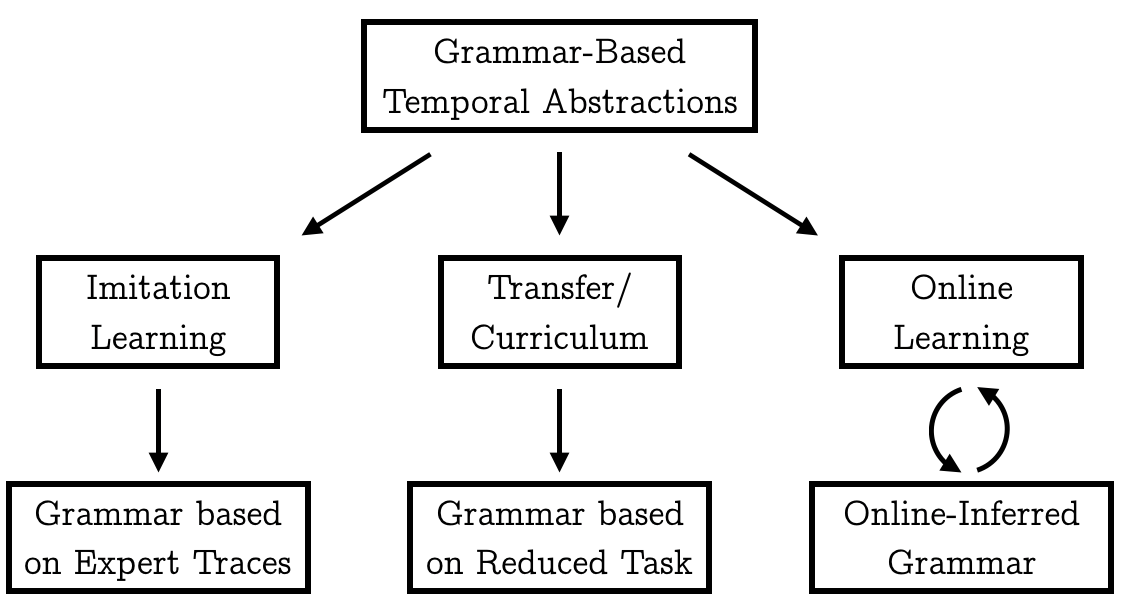
\includegraphics[width=0.475\textwidth]{figures/concept_applications.png}
    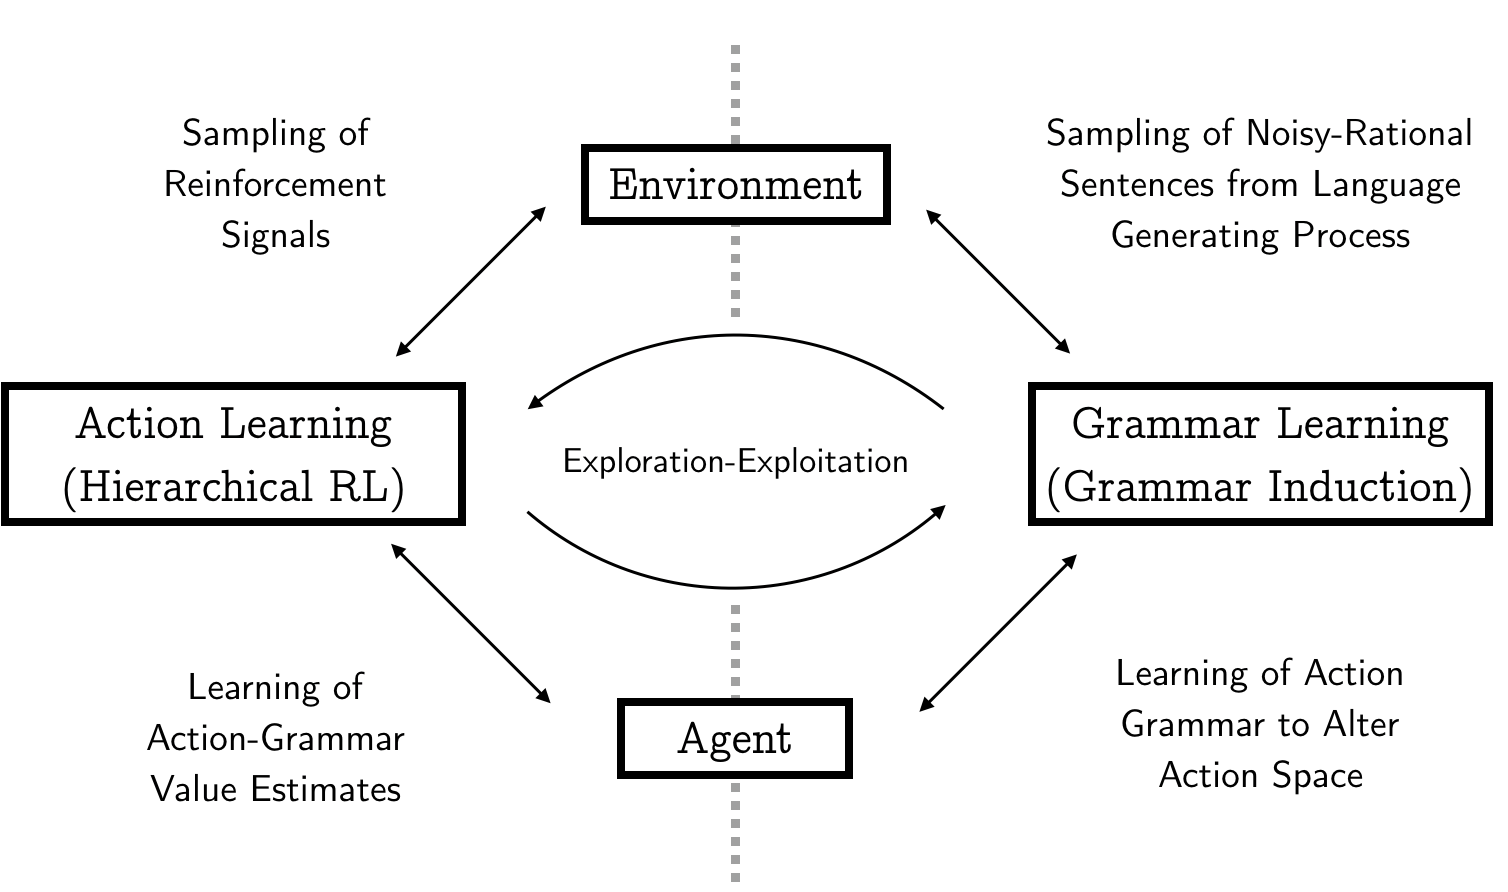
\includegraphics[width=0.475\linewidth]{figures/concept_al_gl.png}
    \caption{Action Grammars for HRL. \textbf{Left.} Applicability of expert action grammars for imitation, transfer and online learning. \textbf{Right.} Online-inferred action grammars alternation loop. The procedure consists of alternating updates of the grammar estimate and a refinement of the corresponding "action grammar" value estimates}
    \label{fig:loop_ag}
\end{figure}

In the following we outline how a general grammar-augmented Reinforcement Learning procedure provides semantically meaningful solutions to key problems in RL (see left part of figure \ref{fig:loop_ag}).
We proceed in the following manner: First, we summarize the current state of sub-structure discovery for HRL and review the required technical background. Afterwards, we introduce our proposed framework and outline how grammar-based temporal abstractions are able to provide efficient, effective and interpretable sub-structures. Our experiments highlight the usability of the action grammars framework for imitation learning and transfer learning given an expert grammar. Furthermore, we display strong results of an online version which iteratively refines grammar and value estimates. 

%--------------------------------------------------------------------
\section{Related Work}

We are not the first to infer hierarchical structure in subgoal achievement problems. More specifically, the option discovery problem deals with the question of how to construct a set of options \citep{Sutton_1999} that captures the hierarchical structure between sub-regions of the core MDP.
Roughly speaking the current state-of-the-art approaches can be categorized in three main pillars:
First, graph theoretic \citep{Hengst_2002, Menache_2002, Mannor_2004, Simsek_2004b} and visitation-based \citep{Mcgovern_2001, Stolle_2002, Simsek_2004b} approaches aim to identify bottlenecks. Bottlenecks are regions in the state space which characterize successful trajectories. This work, on the other hand, identifies patterns solely in the action space and does not rely on rewardless exploration of the state space.
%
Gradient-based approaches, on the other hand, discover parametrized temporally-extended actions by iteratively optimizing an objective function such as the estimated expected value of the log likelihood with respect to the latent variables in a probabilistic setting \citep{Daniel_2016} or simply the expected cumulative reward in a policy gradient context \citep{Bacon_2017, Smith_2018}. Grammar induction infers patterns without supervision solely based on a compression objective. The resulting parse tree provides an interpretable structure.
%
Finally, multi-layer \citep{Bakker_2004, Vezhnevets_2017, Florensa_2017} approaches attempt to split the goal declaration and goal achievement across different stages and layers of the learning architecture. Usually, the top level of the hierarchy specifies goals in the environment while the lower levels have to achieve such. Such architectures lack sample efficiency and easy interpretation. Our context-free grammar-based approach, on the other hand, requires few rollout traces and can generalize to more difficult task-settings. 

%--------------------------------------------------------------------
\newpage
\section{Technical Background}

\textbf{Temporally-Extended Actions.} Semi-Markov Decision Processes (SMDP) extend the classical Markov Decision Process setting to incorporate not only environmental uncertainty but also time uncertainty. Instead of dealing with a Dirac waiting distribution, the time between individual decisions is modeled as a random variable, $\tau \in \mathbb{Z}_{++}$. It is described by the probability distribution $P(s', \tau| s, m)$  which characterizes the the joint likelihood of transitioning from state $s \in \mathcal{S}$ into state $s'$ in $\tau$ time steps given action $m$ was pursued. Thereby, SMDPs allow one to elegantly model the execution of actions which extend over multiple time-steps (e.g. sequences of primitive actions or sub-policy execution). Multiple different hierarchical action structures have been proposed \citep{McGovern_1997, Sutton_1999, Parr_1998b, Dayan_1993}. In this work we focus on the most simplest, namely macro-actions. Simply put, a macro-action, $m \in \mathcal{M}$ specifies the sequential and deterministic execution of multiple ($\tau_m$) primitive actions. Let $r_{\tau_m} = \sum_{i=1}^{\tau_m} \gamma^{i-1} r_{t+i}$ denote the accumulated and discounted reward for executing a macro. Value estimates can then be updated using SMDP-Q-Learning \citep{Parr_1998a} in a model-free manner:

$$Q(s, m)_{k+1} = (1-\alpha) Q(s, m)_k + \alpha \left( r_{\tau_m} + \gamma^{\tau_m} \max_{m' \in \mathcal{A} \cup \mathcal{M}} Q(s', m')_k \right)$$  

In order to increase sample efficiency, it is recommended to perform intra-macro updates for each state transition tuple $\{<s,a,r,s'>\}_{\tau_m}$ within the macro execution.
The experience replay buffer and DQN objective can also easily be refined to the case of temporally-extended actions:

$$L(\theta) := \mathbb{E}_{s,m,r_{\tau_m},s', \tau \sim D_{\tau_m}} [(r_{\tau_m} + \gamma^{\tau_m} \max_{m' \in \mathcal{A} \cup \mathcal{M}} Q(s',m';\theta^-) - Q(s,m; \theta))^2] $$

\textbf{Context-Free Grammars.} Formal grammars and the theory of computational linguistics study both generating and accepting systems that underlie a language. Given a start symbol $S$, a formal grammar $(\Sigma, \mathbb{N}, S, \mathcal{P})$ produces an output which is a string of words. The terminal vocabulary $\Sigma$ is a set of terminal elements used to construct the sentences of a language. $\mathbb{N}$ denotes the non-terminal vocabulary which is a set of elements only used in the process of deriving a sentence.
%$V^\star$, on the other hand, denotes the set of all possible strings of possible elements in the vocabulary and $V^+$ the set of all possible strings of possible elements except for the null-string in the vocabulary.
The production rules $\mathcal{P}$ are ordered pairs of strings such that $\alpha \to \beta, \alpha \in V^+, \beta \in V^\star$.
A type-2 grammar \citep{Chomsky_1959a, Chomsky_1959b}, also known as context-free grammar (CFG) is such that the production rules have the following form: 
 
 \vspace{-0.25cm}
 $$A \to \beta \text{  , where   } \beta \neq \lambda \text{   or  } |\beta| \neq 0$$
 
 Since production rules either map from one-to-one, one-to-none or one-to-many they are called context-free. The context of a non-terminal symbol does not influence the production rule \citep{Pastra_2012}.
A context-free grammar that is non-branching and loop-free is called a straight-line grammar \citep{Siyari_2016}. Such grammars are restrictive since they are only capable of generating a single sentence.

The process of inferring a grammar for a language that is consistent with a given sample of sentences is called grammatical inference or grammar induction \citep{Levelt_2008}. The smallest grammar problem \citep{Charikar_2005, Siyari_2016} formalizes the problem of finding the smallest CFG which compresses a string generated by a straight-line grammar. This problem turns out to be NP-hard \citep{Charikar_2005}. Two greedy approximations to the smallest CFG are provided by Sequitur \citep{Manning_1997} and G-Lexis \citep{Siyari_2016b}.
Given a single sentence of the language, Sequitur sequentially reads in all symbols and collects repeating subsequences of symbols into a production rule. Therewhile, the final encoded string is only allowed to have unique bigrams (\textit{Digram Uniqueness}, \citep{Manning_1997}) and production rules must be used more than once in the derivation of the string (\textit{Rule Uniqueness}, \citep{Manning_1997}).
In order to overcome Sequitur's problem of noise overfitting, $k$-Sequitur \citep{Stout_2018} has been proposed. Instead of replacing a bigram with a rule if the bigram occurs twice, it has to occur at least $k$ times. As $k$ increases the discovered CFG grammar becomes less and less sensitive to overfitting noise and the resulting grammar is more parsimonious in terms of productions. 
Lexis \citep{Siyari_2016b} provides an optimization-based alternative which iteratively constructs a directed acyclic graph (DAG), the so-called Lexis-DAG. Starting from a trivial graph which connects a set of target sentences with the set of elements in the terminal vocabulary, the Lexis-DAG is constructed by adding intermediate nodes. The indirect objective is to minimize a cost function (e.g. number of concatenations or DAG edges) while imposing that the constructed graph satisfies a set of Lexis-DAG properties. Again, this problem by itself is NP-hard. G-Lexis, the greedy algorithmic implementation, searches for substrings that will lead to a maximal reduction in the cost, when added as new intermediate node.


%--------------------------------------------------------------------
\newpage
\section{Context-Free Action Grammars}

 Action sequences as well as communication by the means of words both convey meaning and are goal-directed. Both consist of hierarchical structures and are conditioned by the environment in which they are uttered in. The crucial assumption that connects linguistics with eager behavior is as follows: 

\begin{assumption}
	Observed episodic behavior (with trajectory $\vartheta = \{\vartheta_1, \dots, \vartheta_T\}$ where $\vartheta_t =\{s_t, a_t\}$) can be equivalently viewed as sentences sampled from the language, $L(G)$ with $G \sim \pi|E$.
\end{assumption}

Let us assume that the optimal policy of a Reinforcement Learning agent is hierarchically structured (i.e. with repeating sequences of actions) for a specific environment $E$. The optimal policy $\pi^\star$ then consists of a hierarchy of subgoal achievements which increase in sequential difficulty when moving up the hierarchy.
We define the terminal vocabulary $\Sigma$ to consist of the primitive action space $\mathcal{A}$, hence $\Sigma = \mathcal{A}$.
A trajectory obtained from traversing the current policy $\pi$ is viewed as a sample from the language generated by the grammar $L(\pi|E)$. We write  $\vartheta^i \sim L(\pi|E)$ for $i = 1, \dots N_g$ trajectories. Each trajectory has an individual length denoted by $T_{i}$. Given a set of trajectories, $\vartheta^1, \dots \vartheta^{N_g}$, a context-free grammar estimate $\hat{G}$ can be inferred. The resulting production rules can be transformed into macro-actions by recursive flattening. We augment the action space of the HRL agent, e.g. $\mathcal{A}^{\hat{G}} = \mathcal{A} \cup \mathcal{M}^{\hat{G}}$. Depending on the nature of the grammar compressed traces, the HRL agent can utilize the resulting semantically-augmented action space in different ways:

\textbf{Learning with Expert Grammar and Transfer Grammar.} If the traces $\vartheta^i$ are sampled from the language $L(\pi^\star|E)$ generated by the optimal policy, the agent can use the resulting grammar and flattened macros in an imitation learning setting. Furthermore, an agent faced with learning a sequence of tasks with increasing difficulty can make use of the optimal grammar for the previous task. Thereby, skills which are universal to all tasks do not have to be re-learned at every tasks. Instead, the relevant sequential behavior is already captured by the grammar macro. 

\begin{wrapfigure}{r}{0.53\textwidth}
  \begin{center}
    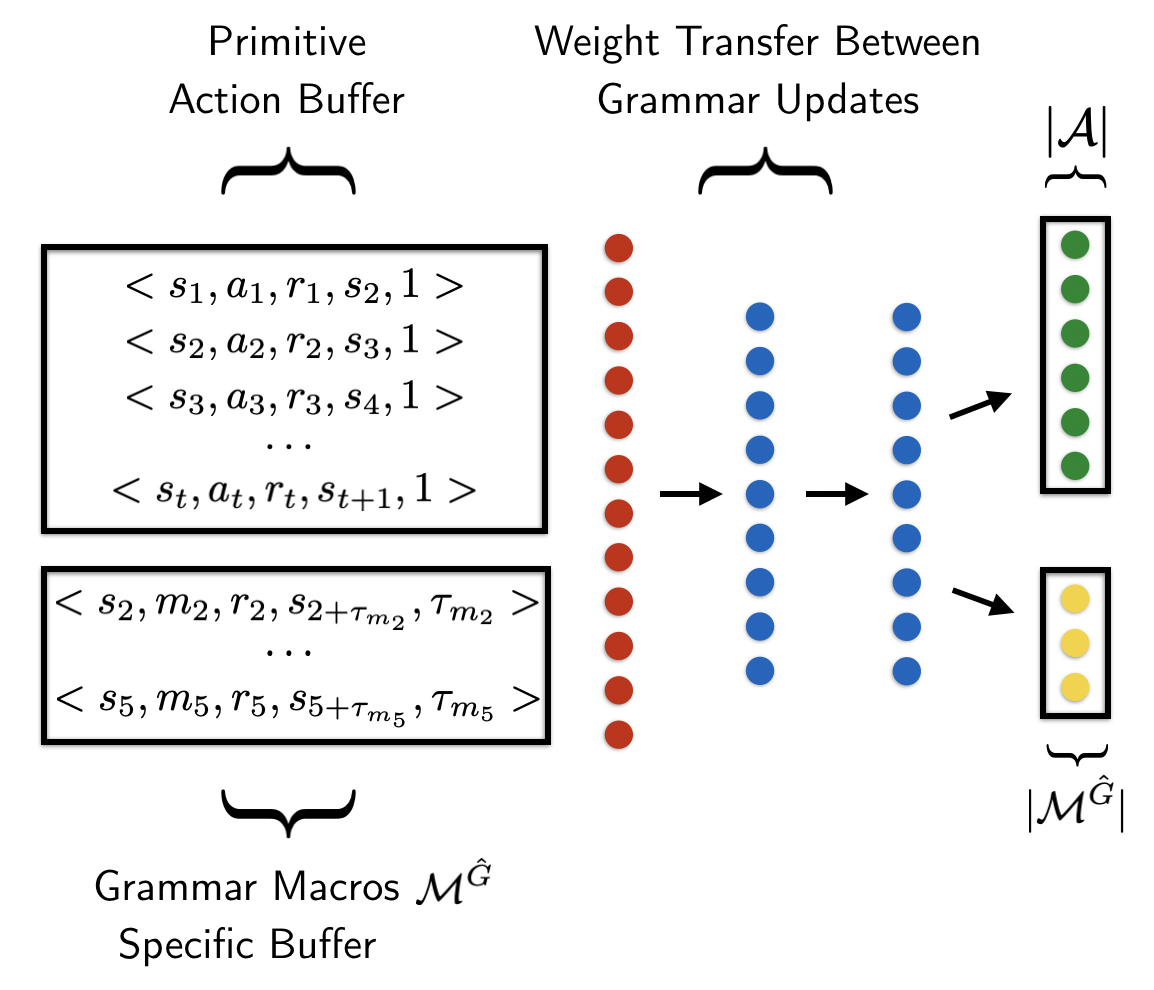
\includegraphics[width=0.52\textwidth]{figures/ag_dqn_buffer}
  \end{center}
  \caption{Online Grammar DQN with adaptive output.}
  \label{fig:online_ag_dqn}
\end{wrapfigure}

\textbf{Learning with Online Inferred Grammars.} The previous approach relied on a single set of static expert traces from which the agent once infers a grammar and then continues to perform SMDP-Q-Learning. Another approach is to alternate between a stage of grammar learning based on self-rollouts and a stage of action value refinements (see right part of figure \ref{fig:loop_ag}). If the episode successfully terminated, the grammar inference process identifies repeating patterns that led to successful goal achieving experiences. By extracting these patterns and redefining them as temporally-extended actions, we can additionally \textit{reflect and store} the progress made not only in the value estimate but also in the augmented action space. 
A natural question then becomes how to transfer values between two stages of value learning? In order to approximately preserve value estimates, we make use of transfer learning. 
More specifically, the classical DQN architecture can be altered as follows (see figure \ref{fig:online_ag_dqn}): In order to accommodate the variable set of grammar-inferred skills the size of the DQN output layer has to be updated after every grammar learning step yielding new macro-actions. By transferring or keeping the previously learned parameters fixed between action space augmentation, the agent can utilize the previously learned value characteristics. The weights of the final can then be relearned during the value learning stage. Again, we highlight the necessity of intra-macro learning in order to achieve sample efficient learning.
Furthermore, it is necessary to maintain a separate experience buffer system in order to store transition tuples specific to inactive previously inferred macro actions.  
Finally, we highlight the importance of adapting the hyperparameters of the grammar inference algorithm. The length of the sampled trace is going to increase or decrease over the course of the learning procedure. Hence, regularization parameter of the $k$-Sequitur grammar inference algorithm has to be changed accordingly.

%--------------------------------------------------------------------
\newpage
\section{Experiments}

The goal of the experimental section of this work is to answer the following questions: (1) Does a grammar learned on optimal policy traces allow for rapid imitation learning? (2) Can CFG grammars be used in order to enhance curriculum as well as transfer learning? (3) Is online grammar inference and action space adaptation able to structure the exploration process of the HRL agent?

In order to illustrate our results we choose the $N$-disk Towers of Hanoi (ToH) environment (see left part of figure \ref{fig:hanoi}). The general game setting for $N$ disks is as follows: In every episode of the game the agent is initialized in the tuple $(1)_{i=1}^N$. At each point in (discrete) time the agent transitions between states with the help of the following moves:  $\mathcal{A} = \{a:(1,2); b:(1,3); c:(2,1); d:(2,3); e:(3,1); f:(3,2)\}$. The agent maximizes their expected cumulative discounted reward by reaching the final state $(3)_{i=1}^N$ as quickly as possible. The problem is formulated as a sparse long-term credit assignment problematic. The size of the state space, on the other hand, grows exponentially, $|S| = 3^N$ (all possible allowed orderings), and the optimal number of moves to solve this game is given by $2^N - 1$. A simple recursive procedure to solve the problem for all states in which the top $N-n$ disks are already correctly ordered on the third pole is given by:

\begin{enumerate}
	\item Move $n-1$ disks from source pole to auxiliary pole
	\item Move the $n$-th disk from source pole to target pole
	\item Move the $n-1$ disks that we left on auxiliary pole onto target pole
\end{enumerate}

 \begin{minipage}{\textwidth}
  \begin{minipage}[b]{0.49\textwidth}
    \centering
    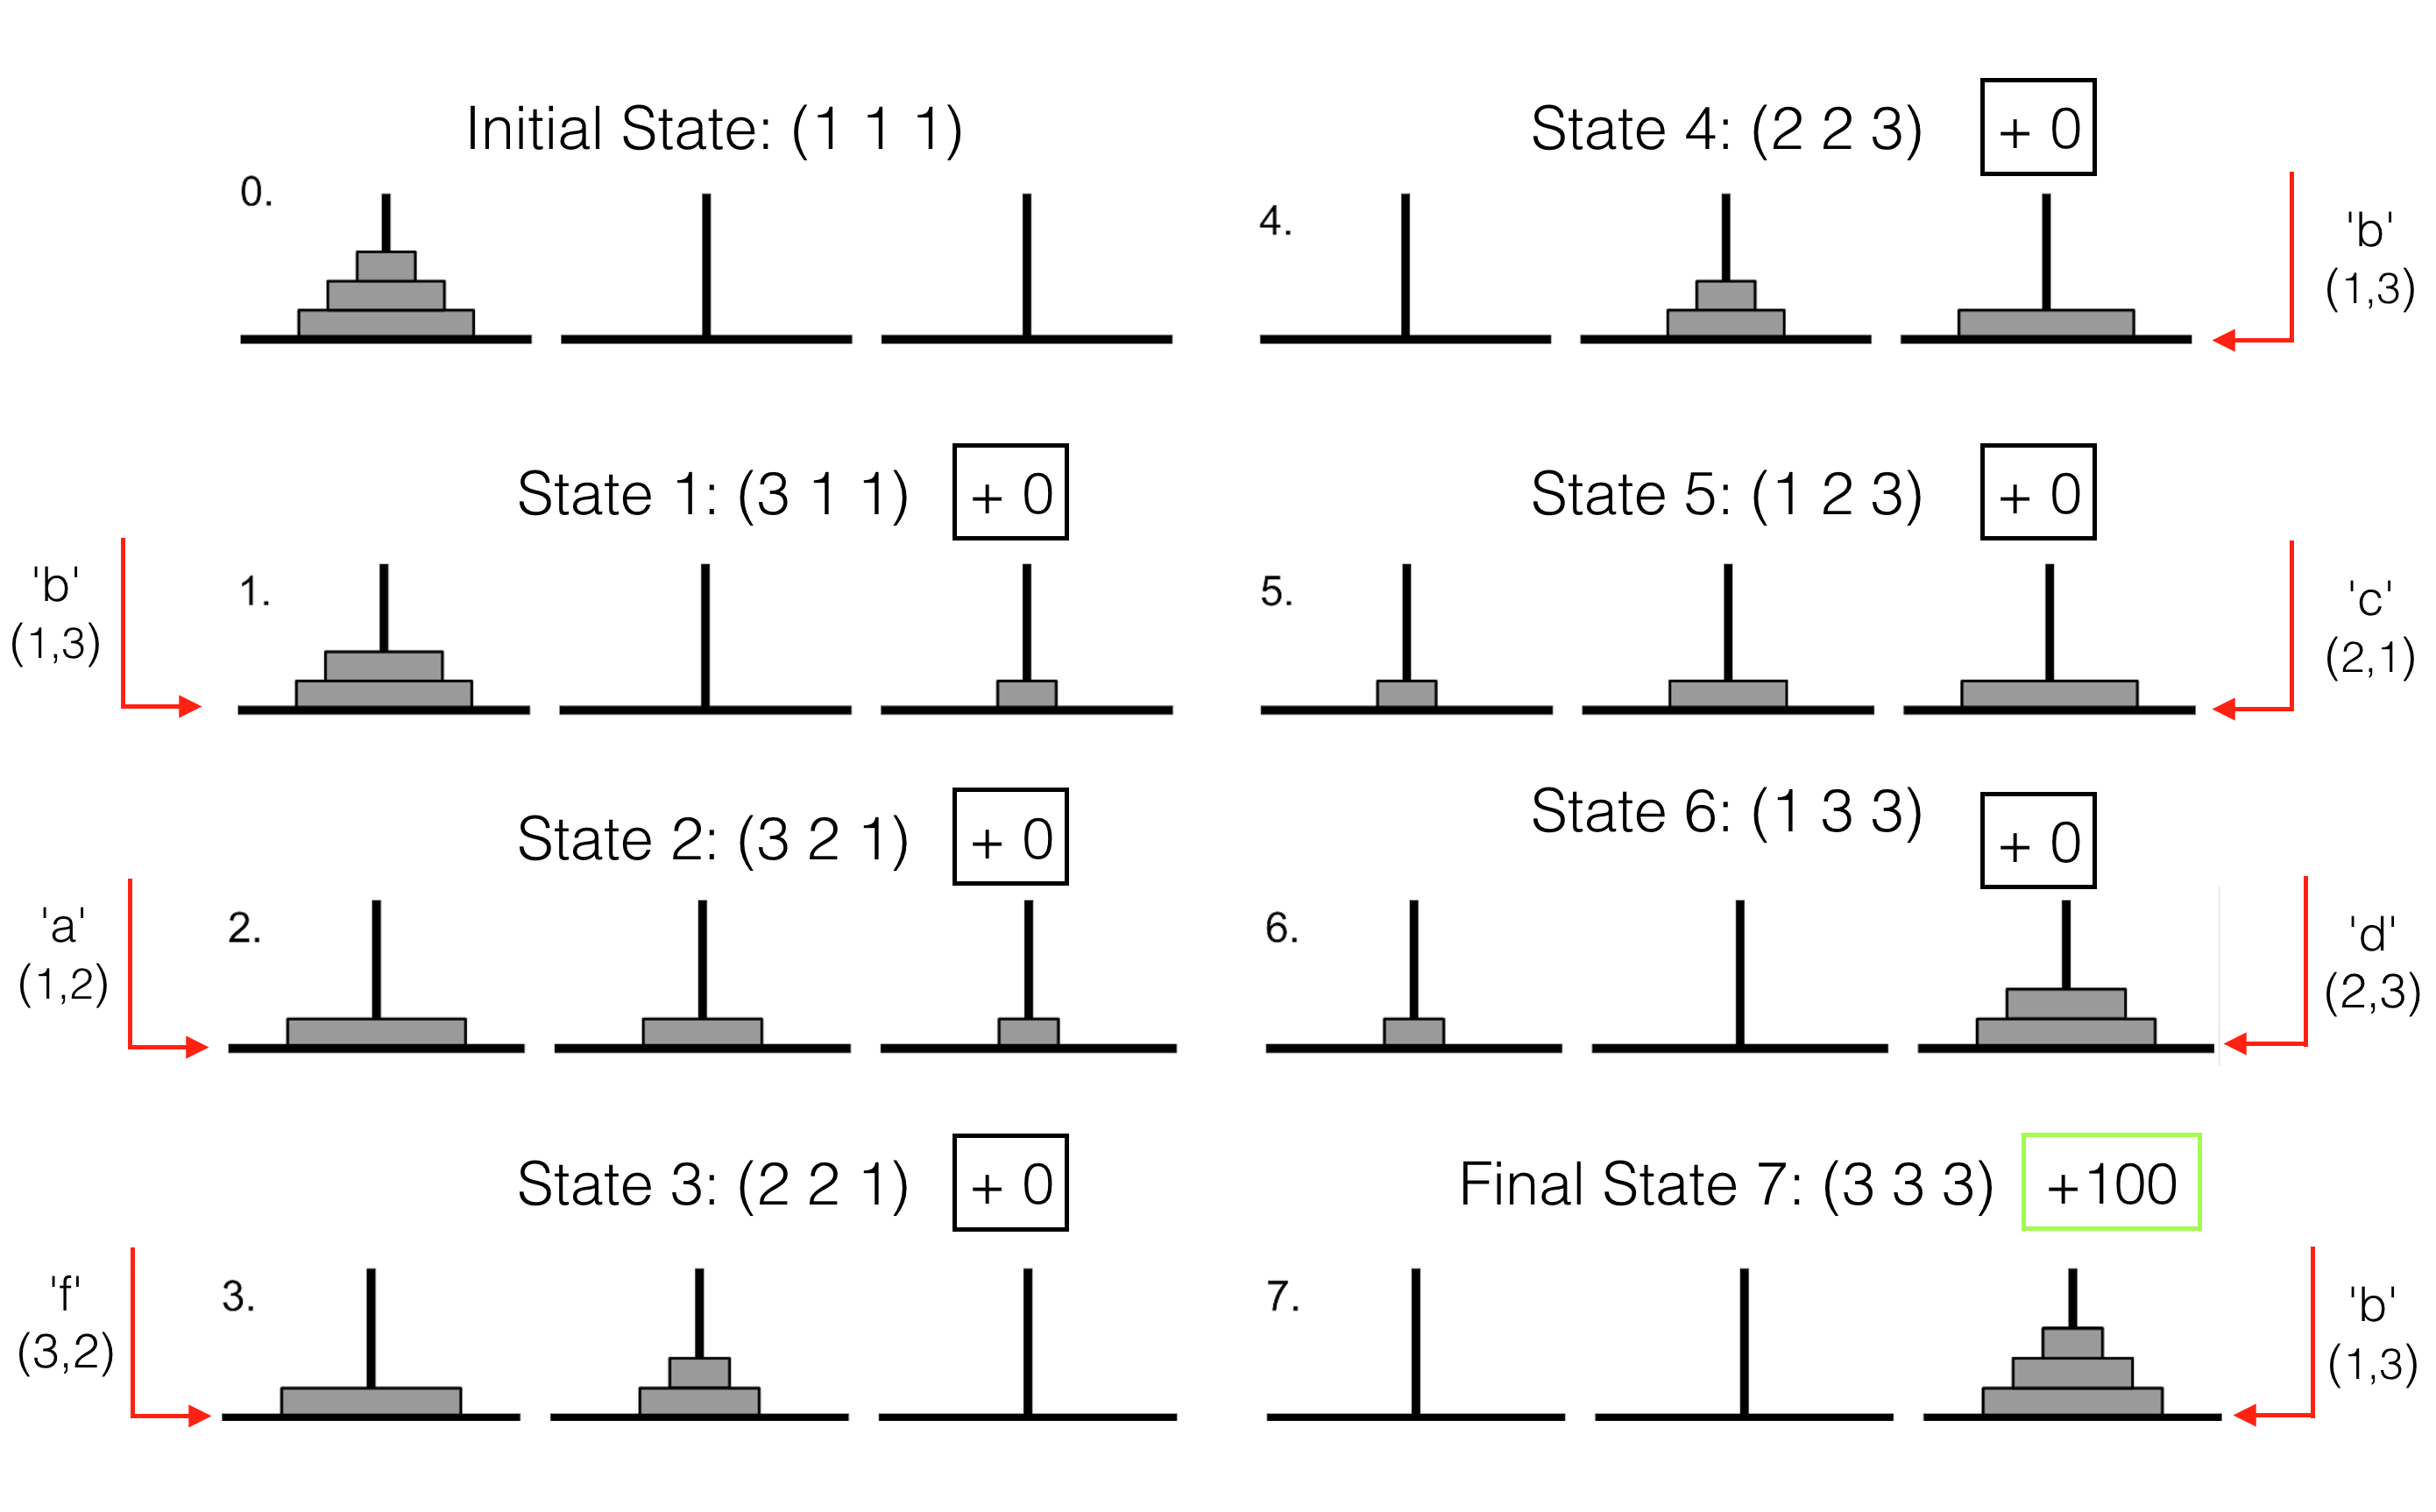
\includegraphics[width=\textwidth]{figures/hanoi_problem.png}
    \captionof{figure}{RL Formulation of the ToH Problem}
    \label{fig:hanoi}
  \end{minipage}
  \hfill
  \begin{minipage}[b]{0.49\textwidth}
    \centering
    \begin{tabular}{c | c c | c c } % centered columns (4 columns)
\hline\hline %inserts double horizontal lines
 \multicolumn{5}{c}{Trace ($\vartheta$): bafbcdbafecfbafbcdbcfecdbafbcdb
} \\
\hline\hline
  & \multicolumn{2}{c}{$2$-Sequitur} & \multicolumn{2}{c}{G-Lexis}\\
\hline
 $\vartheta^{enc}$ & \multicolumn{2}{c}{BCDfBEfDdBb} & \multicolumn{2}{c}{BbafecfBbcfecdBb}\\
 $\frac{|\vartheta^{enc}|}{|\vartheta|}$ & \multicolumn{2}{c}{0.355} & \multicolumn{2}{c}{0.516}\\
 %$\frac{\mathcal{H}(\vartheta^{enc})}{\mathcal{H}(\vartheta)}$ & \multicolumn{2}{c}{1.0702} & \multicolumn{2}{c}{1.3613}\\
\hline \hline
$\mathbb{N}$ & PR & $\mathcal{M}^{2-Seq}$ & PR & $\mathcal{M}^{G-Lex}$\\ % inserts
\hline % inserts single horizontal line
B & CEd & bafbcd & - & bafbcd\\
C & - & baf &&  \\
D & - & ec &&  \\
E & - & bc &&  \\ 
\hline %inserts single line
\end{tabular}
      \captionof{table}{ToH (5 disks) Grammar-Macro Construction}
      \label{table:optimal_grammar}
    \end{minipage}
  \end{minipage}
  
Identifying this underlying hierarchical principle and generalizing between different environments requires the agent to correctly identify their state in the underlying hierarchical action parse tree.
%-----------------------------------
\subsection{Learning with Expert Grammar and Transfer Grammar}


\begin{wrapfigure}{r}{0.5\textwidth}
  \begin{center}
    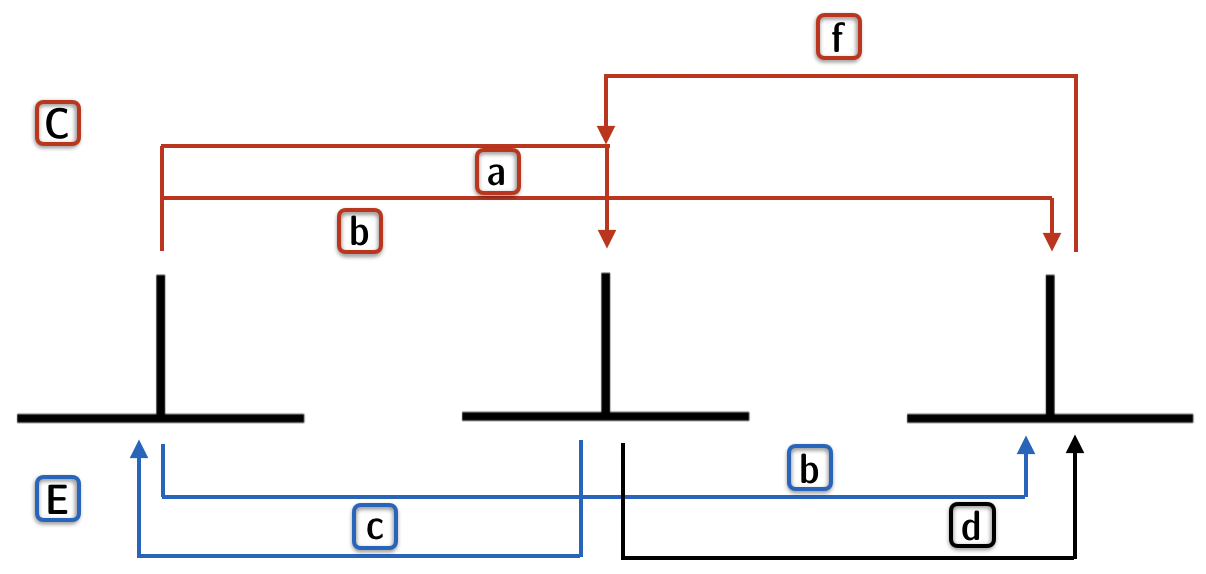
\includegraphics[width=0.49\textwidth]{figures/grammar_macro_viz}
  \end{center}
  \caption{Visualization of the Grammar Macro "B".}
  \label{fig:grammar_macro}
\end{wrapfigure}

Given action sequences of an expert the HRL agent can infer a set of grammar macros and augment their action space. Table \ref{table:optimal_grammar} displays the grammar macros inferred from a trace of the optimal policy using the 2-Sequitur as well as the G-Lexis algorithm. The flattened production rule $B \to CEd \to bafbcd$ is visualized in figure \ref{fig:grammar_macro} and captures the recursive nature learned by the grammar. $C \to baf$ moves two disks on the auxiliary pole, while $E \to bc$ moves a third disk from source to target pole and one disk back onto the source pole. We can then augment the action space of the 5 disk agent in the following way:

$$\mathcal{A}^{\hat{G}} = \mathcal{A} \cup \mathcal{M}^{2-Seq} = \mathcal{A} \cup \{bafbcd, baf, ec, bc\}$$

\begin{figure}[H]
\minipage{0.33\textwidth}
  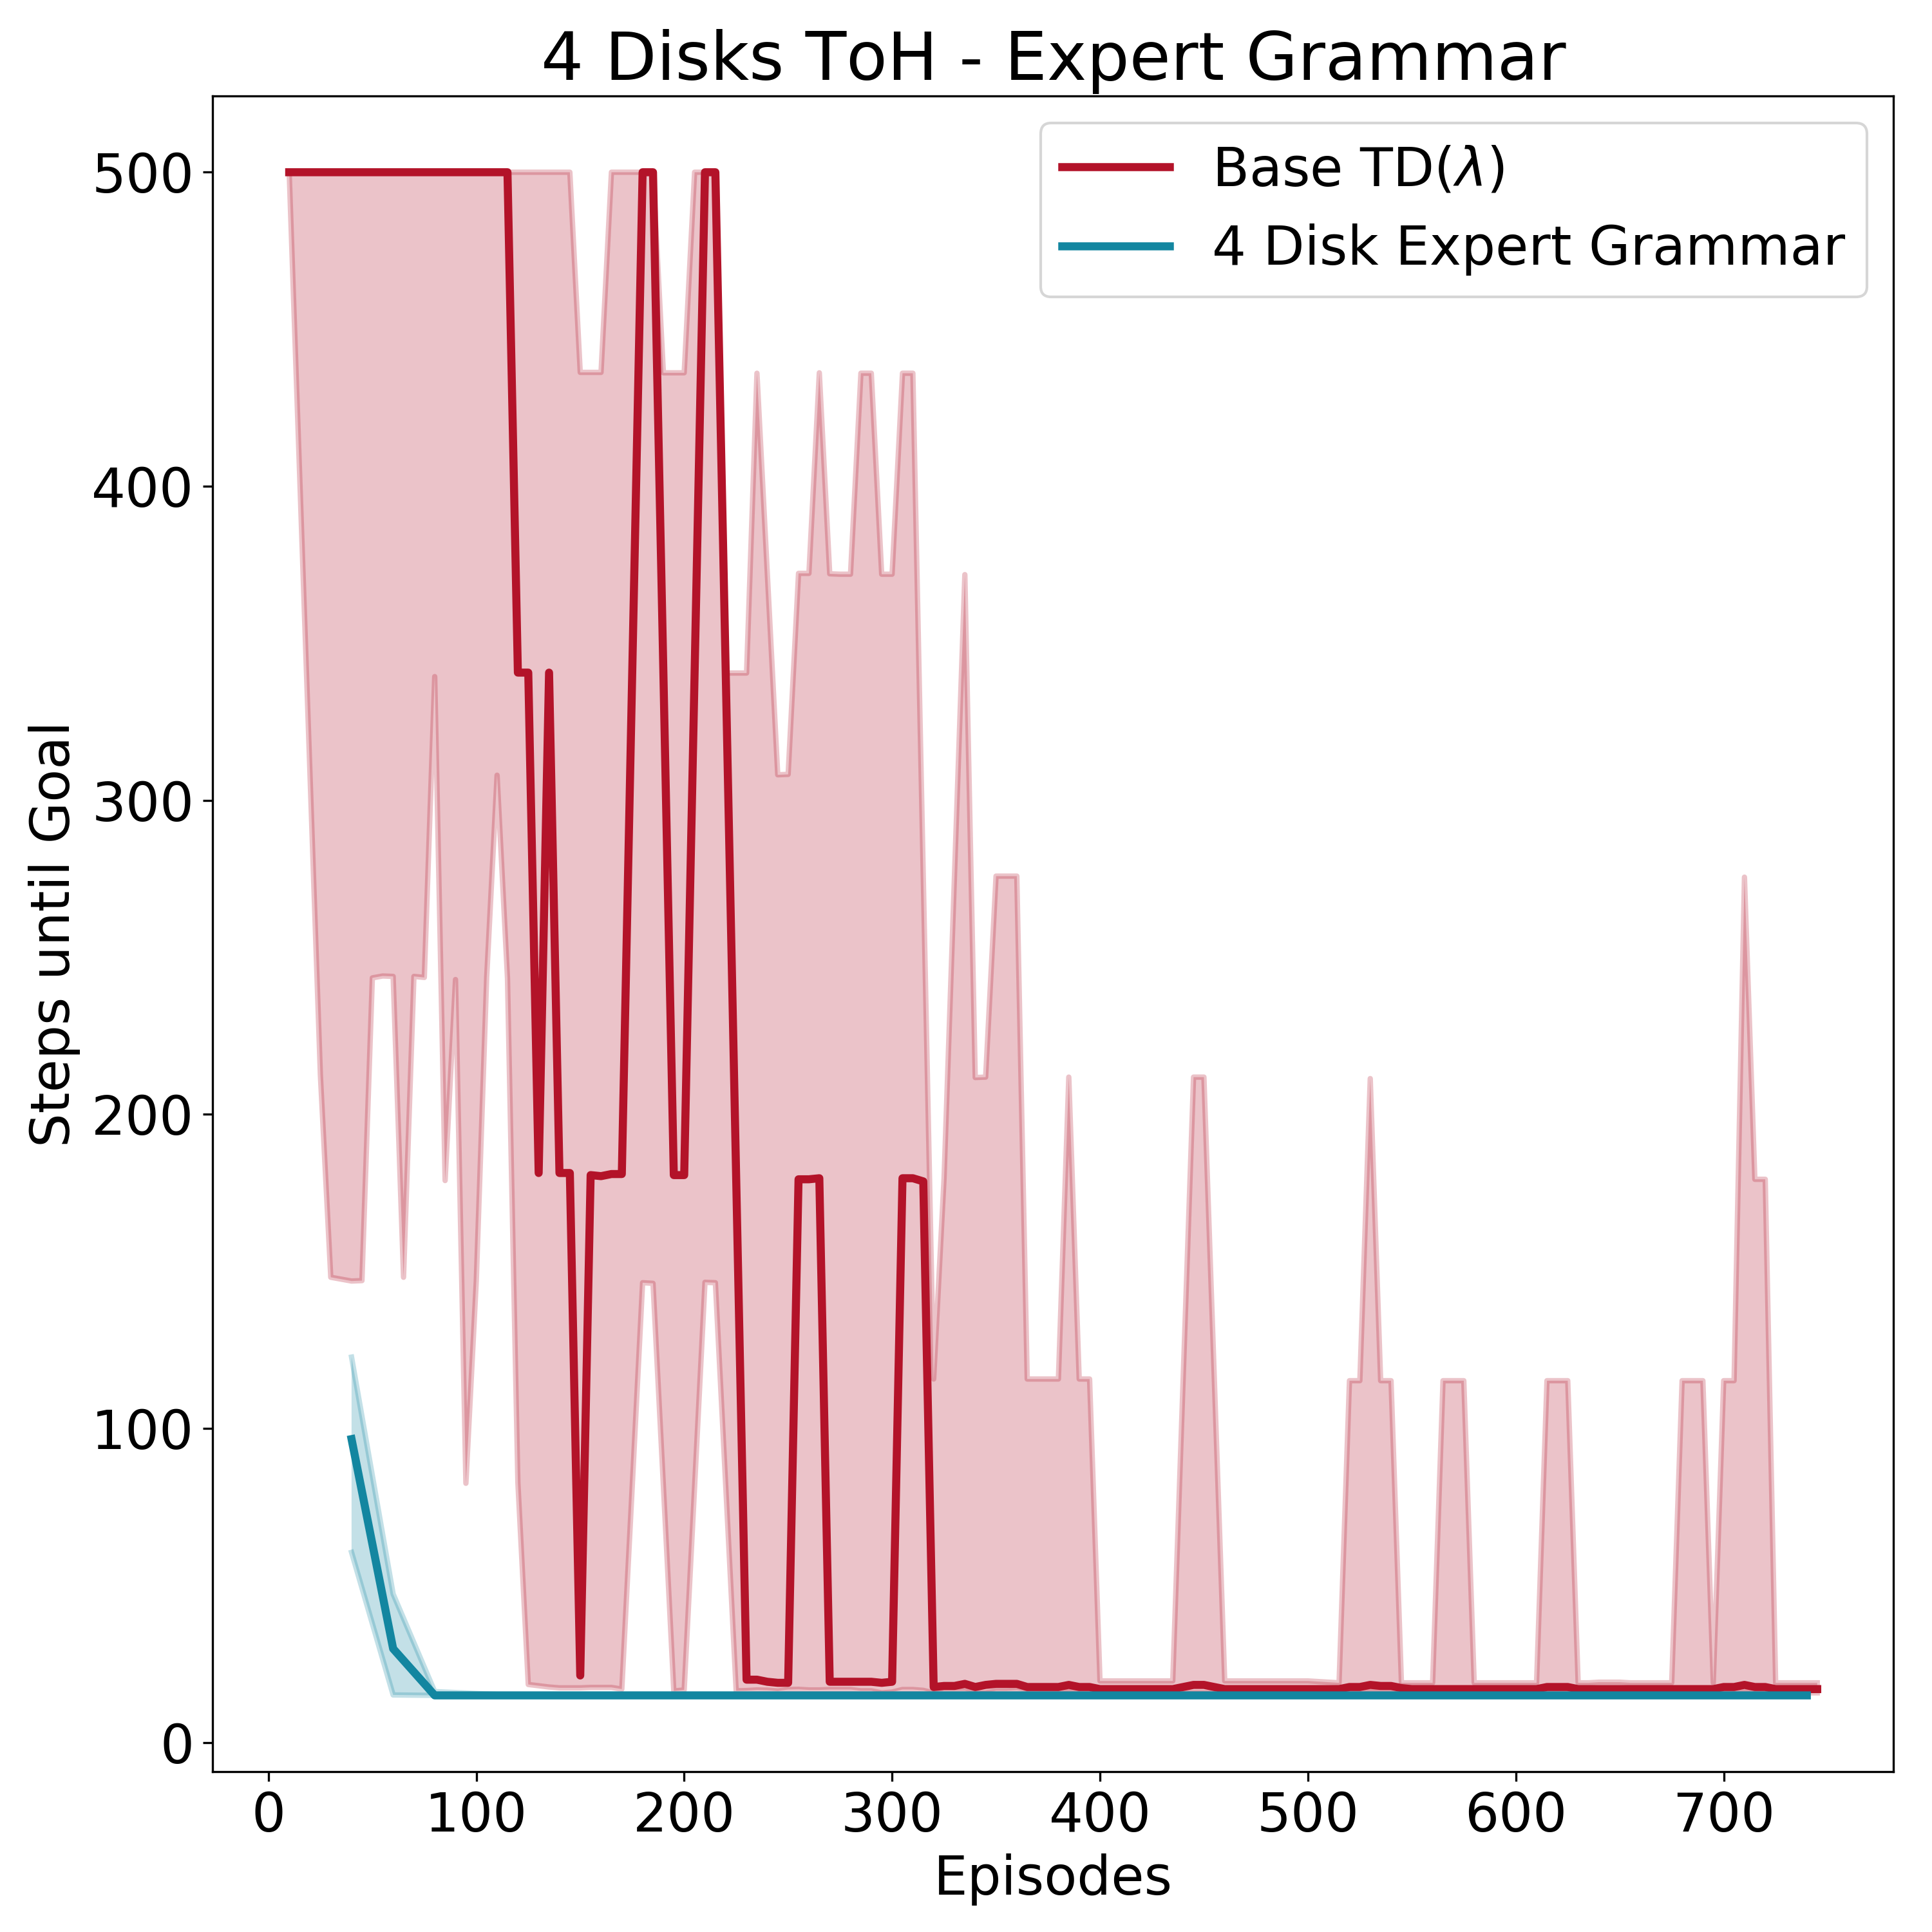
\includegraphics[width=\linewidth]{figures/4_disks_transfer_grammar}
\endminipage\hfill
\minipage{0.33\textwidth}
  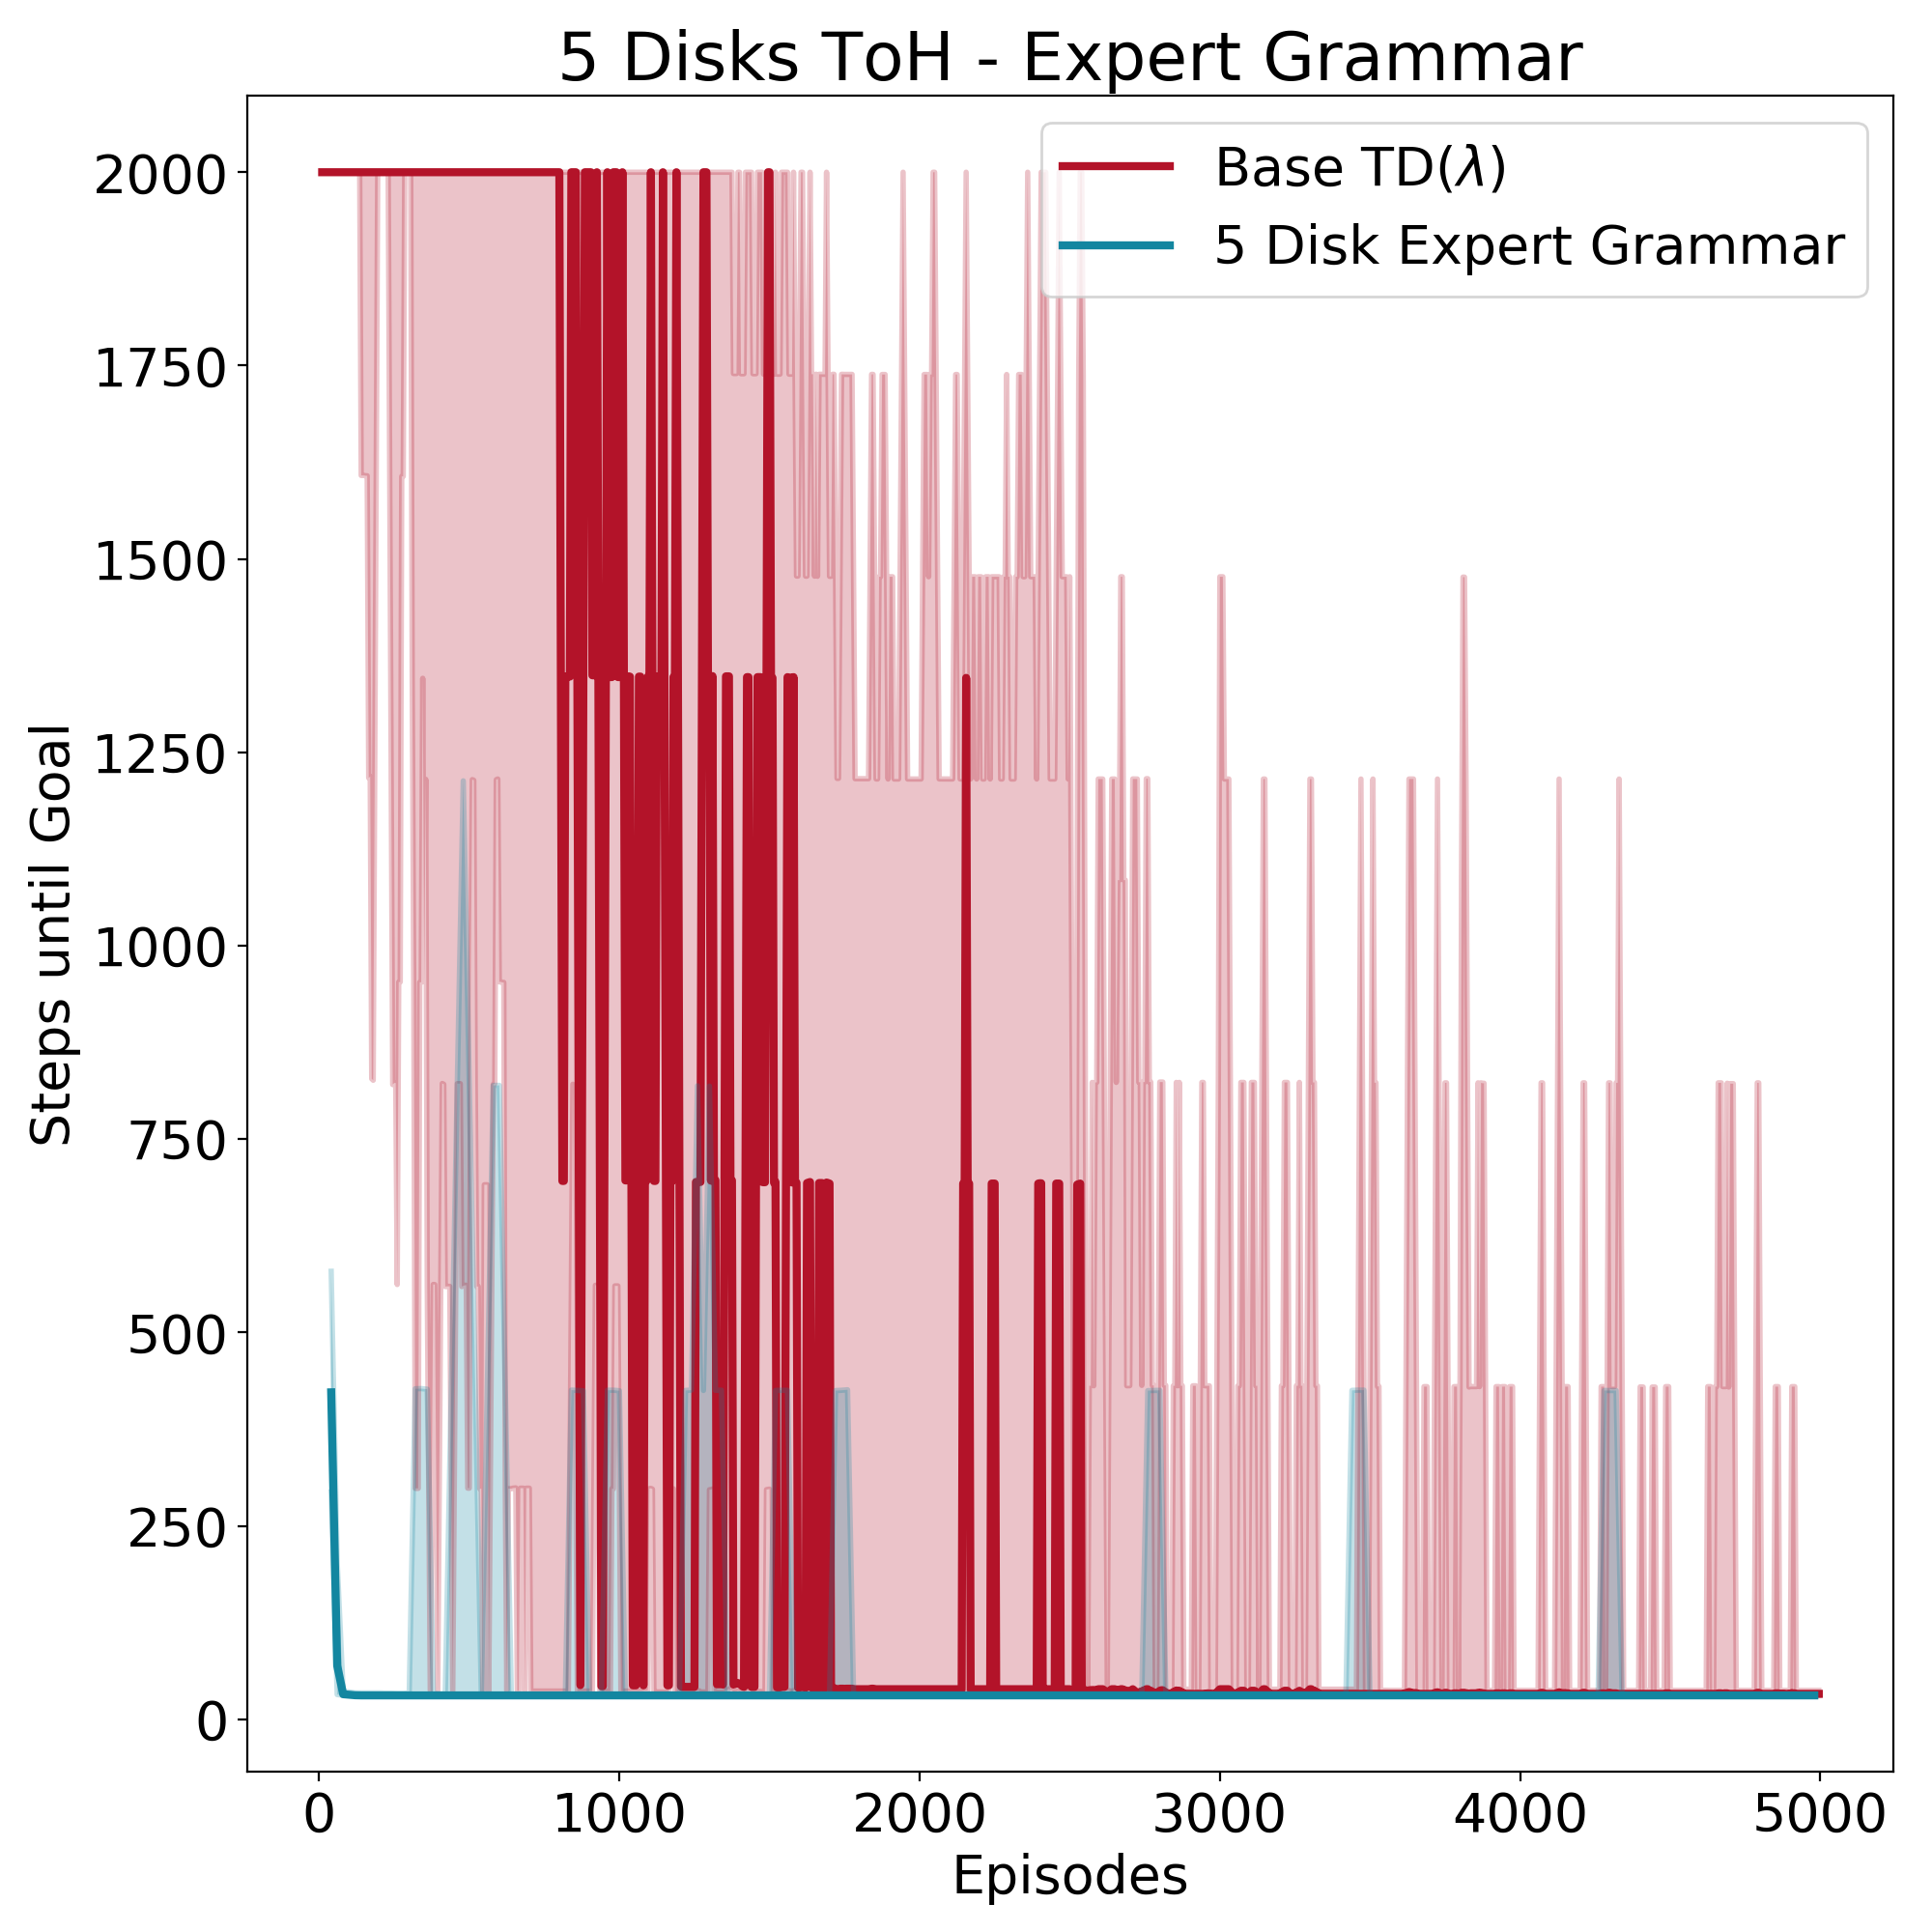
\includegraphics[width=\linewidth]{figures/5_disks_transfer_grammar}
\endminipage\hfill
\minipage{0.33\textwidth}%
  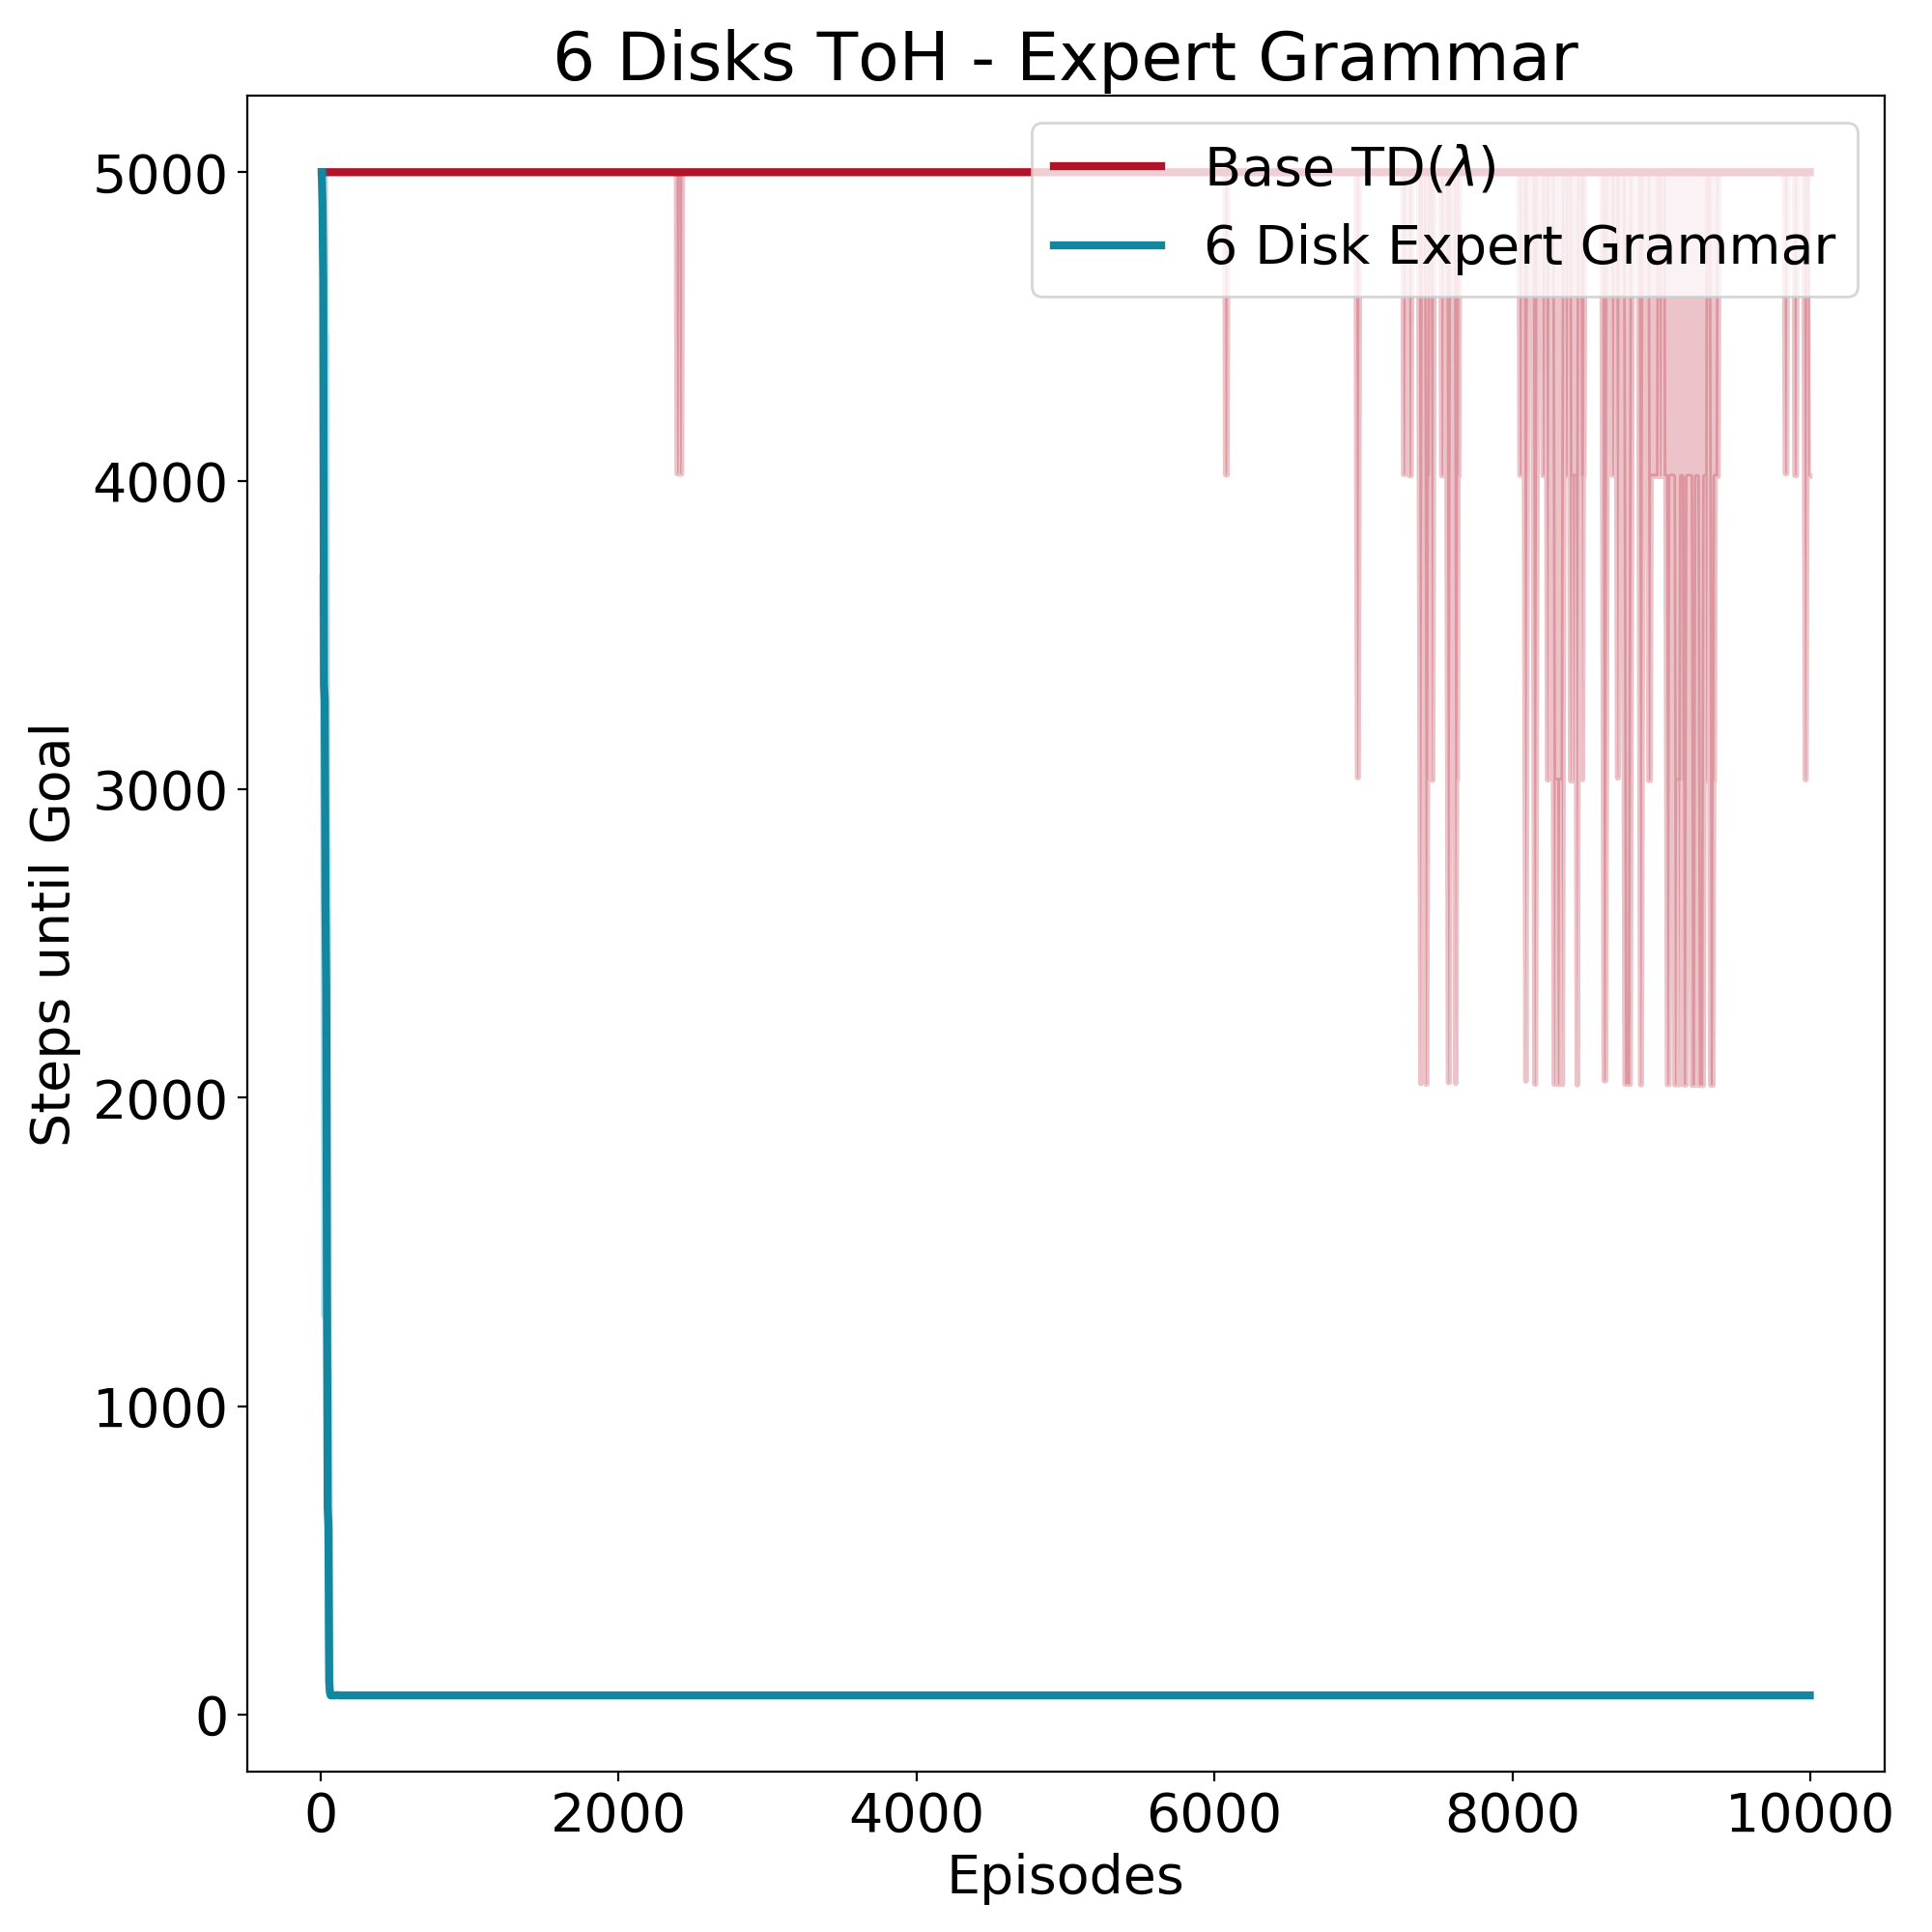
\includegraphics[width=\linewidth]{figures/6_disks_transfer_grammar}
\endminipage
\caption{Learning Results for SMDP-Q-Learning with Expert Grammar Macros for 4, 5 and 6 Disk Environment. Median, 10th percentile and 90th percentile reported over 5 runs.}
\label{fig:expert_grammar}
\end{figure}

Figure \ref{fig:expert_grammar} displays learning results for different SMDP-Q-Learning agents with macro-actions defined by the production rules inferred from a trace of the optimal policy. One can observe that the grammar macros greatly accelerate the learning progress of the agent. Furthermore, the variance of rollouts is greatly reduced due to increased robustness. Instead of using the optimal grammar macros for a specific environment, we are also interested in assessing how well the grammars learned for a more simplistic environment (i.e. $N-1$ disks).  


\missingfigure[figwidth=\textwidth]{Learning Result for Transfer Grammar}
%
%\begin{figure}[H]
%\minipage{0.475\textwidth}
%  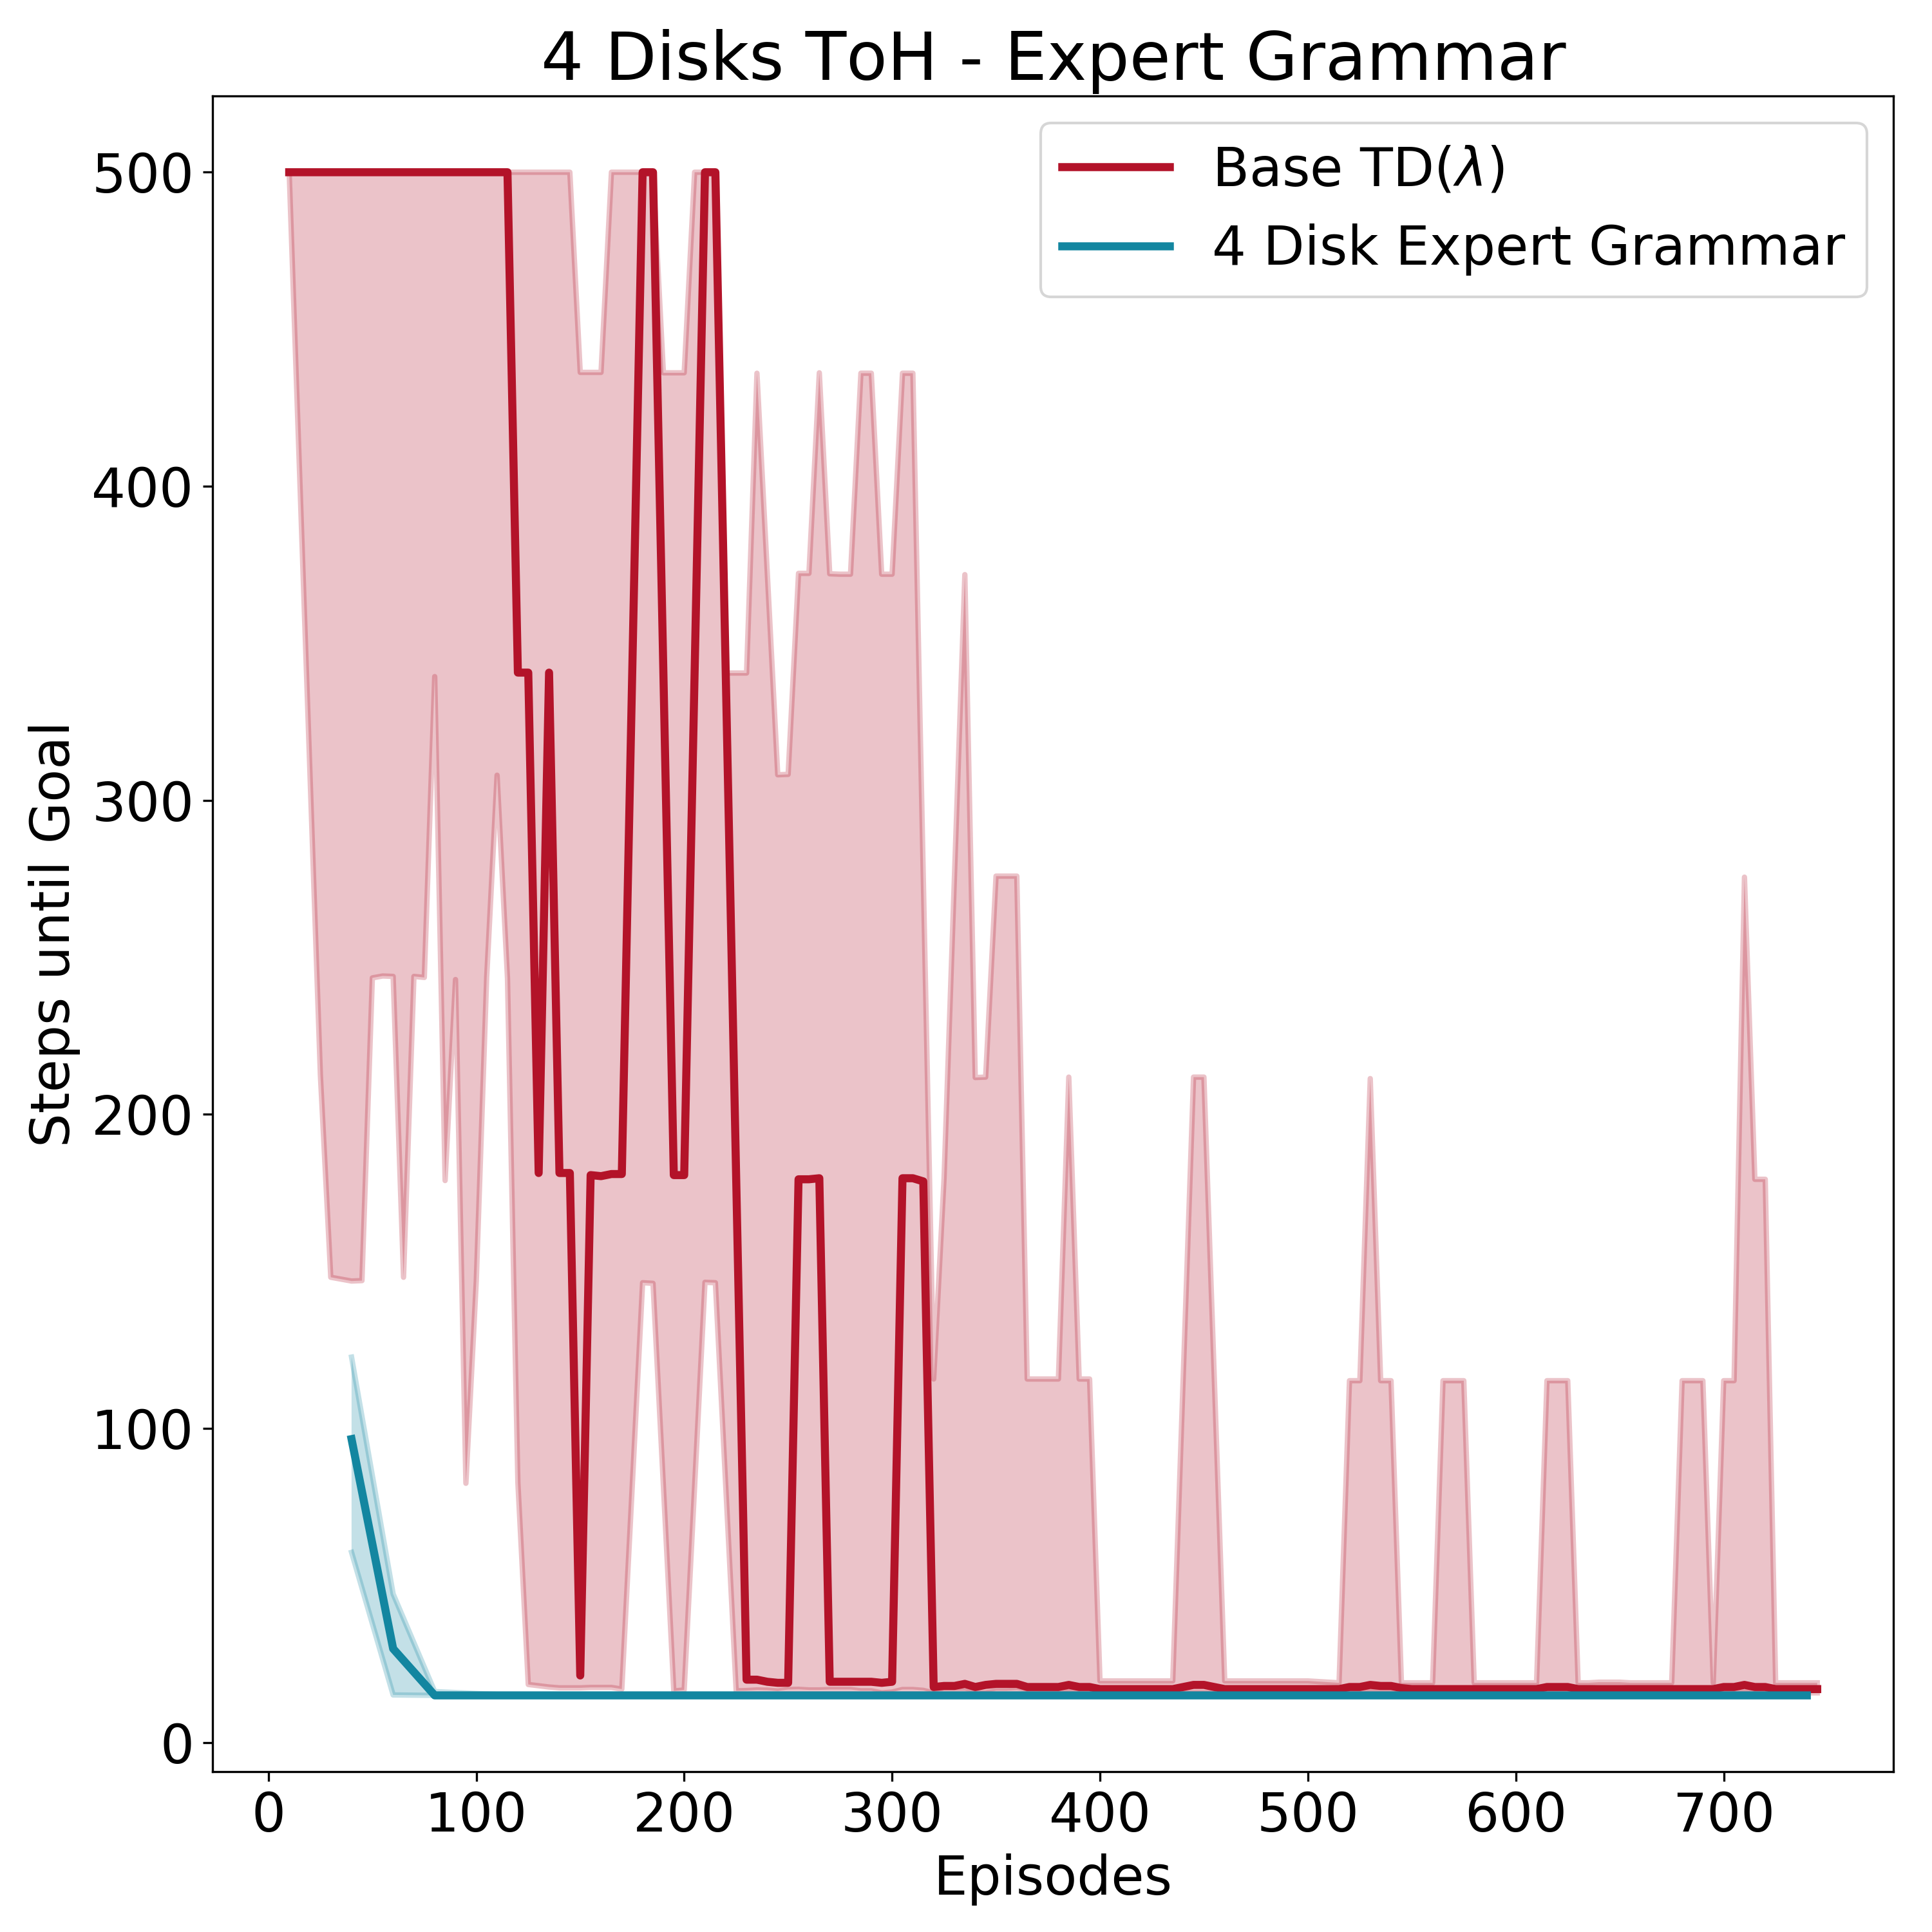
\includegraphics[width=\linewidth]{figures/4_disks_transfer_grammar}
%\endminipage\hfill
%\minipage{0.475\textwidth}
%  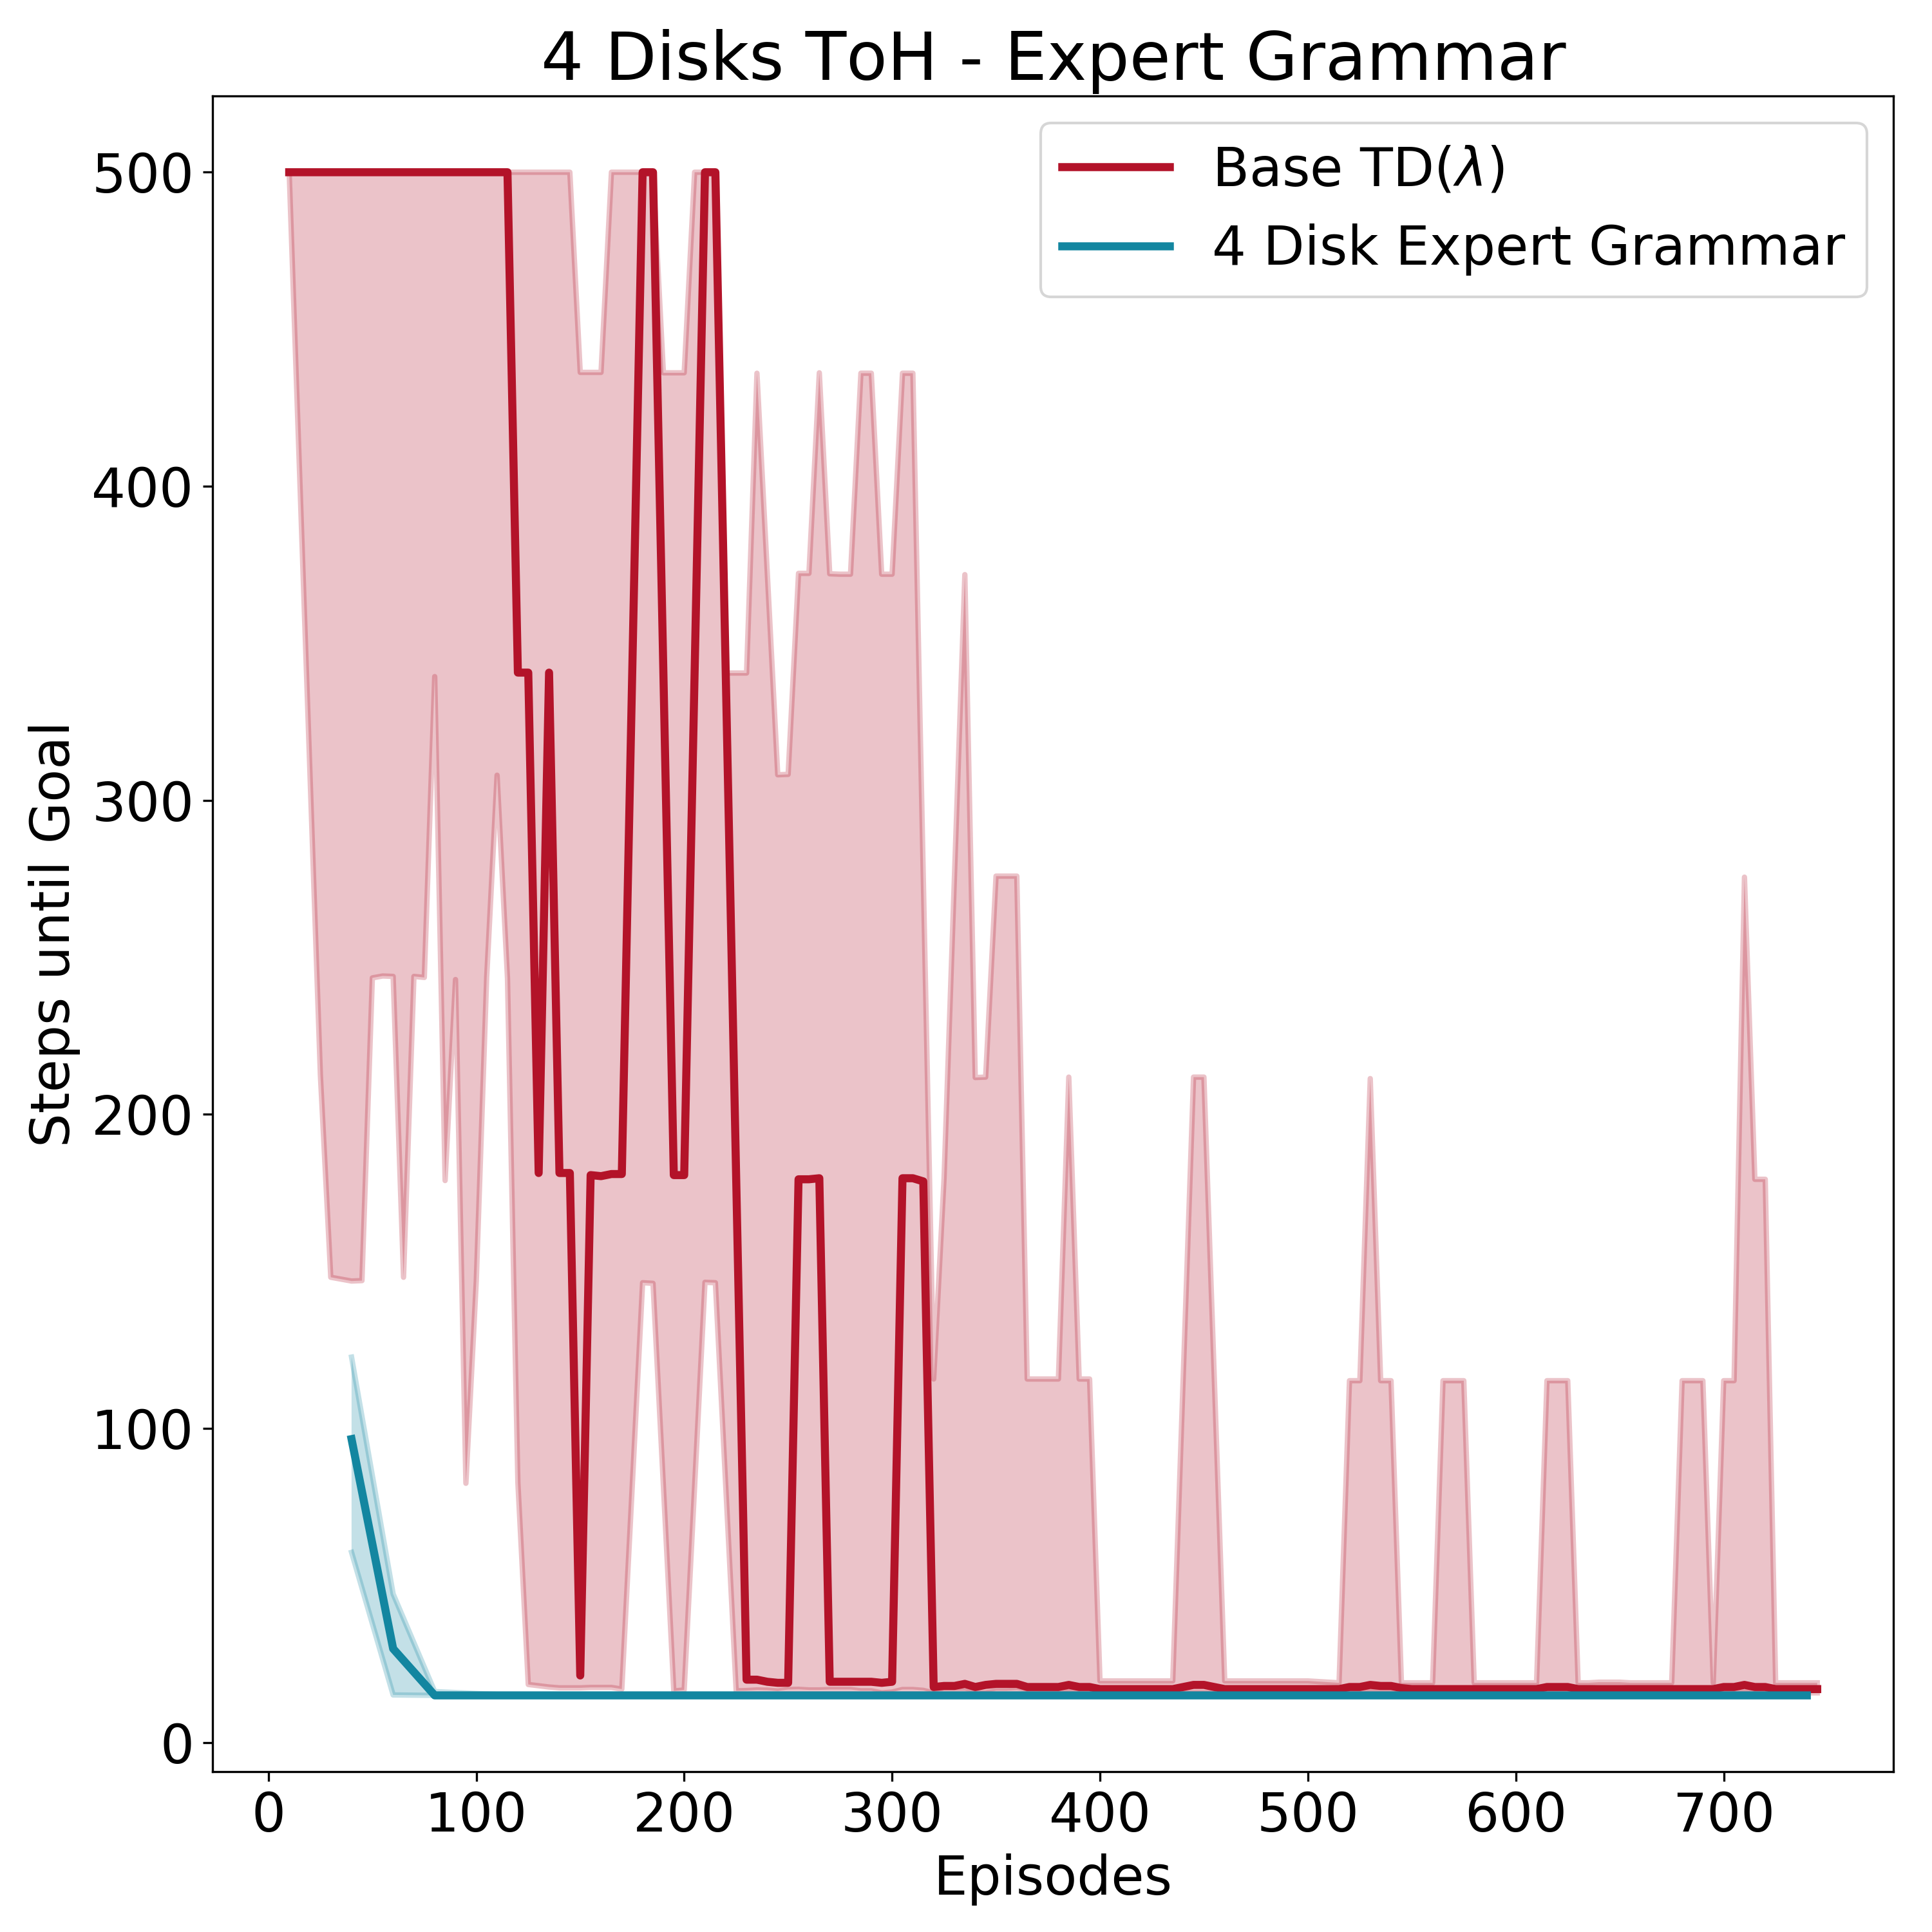
\includegraphics[width=\linewidth]{figures/4_disks_transfer_grammar}
%\endminipage\hfill
%\caption{Learning Results for SMDP-Q-Learning with Transfer Grammar Macros for 5 and 6 Disk Environment. Median, 10th percentile and 90th percentile reported over 5 runs.}
%\label{fig:transfer_grammar}
%\end{figure}


%-----------------------------------
\subsection{Learning with Online Inferred Grammar}

\missingfigure[figwidth=\textwidth]{Learning Result for Online Inferred Grammar}

\rob{Add Grammar DQN experiments.}

%--------------------------------------------------------------------
\newpage
\section{Discussion \& Outlook}

Motivated by a parallelism between the hierarchical generating processes of language and motion, we have derived multiple algorithmic approaches which exploit powerful grammatical inference frameworks to identify temporally-extended actions. At the center of this analysis was the formal notion of Semi-Markov Decision Processes and their capability to model stochastic waiting times between decisions. By sensibly defining temporally-extended actions and abstracting away unnecessary decision points, one is able to overcome the curse of dimensionality. 
In order to validate our proposed framework, we tested both approaches for an imitation learning as well as an online RL task in multiple environments. Our contributions can be summarized as follows:
%
(1) The CFG approach to macro-actions extraction from flat production rules performs very well in both imitation and transfer learning. The agent can easily generalize from the inferred hierarchical structure and is able to increase the action learning speed drastically.
%
(2) Alternating between grammar updates and learning action values is an effective way of both online learning of an optimal grammar as well as an optimal policy. The first grammar extraction and action space augmentation has the largest significant effect in the further learning procedure of the agent. 

In future work we are interested in testing and extending our approach to physical and continuous (joint and velocity-bases state representations, e.g. MoJuCo) domains as well as model-based methods. Formal grammars are especially useful for languages with large terminal vocabulary. So far we have only experimented with discrete action spaces and single agents. \citet{Pastra_2012} note that social interactions of more than one agent can also be formulated within the notion of tool use. Hence, we are interested in possible applications to multi-agent RL  and testing the scalability of our approach to real-life domains.
%
Furthermore, our approach has only attempted to merge grammatical inference with one HRL algorithm. There remain many other promising frameworks such as the Hierarchies of Abstract Machines (HAMs, \citep{Parr_1998a,Parr_1998b}). HAMs define a hierarchy over finite state machines. This could naturally lead itself to automated identification via Hierarchical Hidden Markov Models \citep{Fine_1998}.
%
Future work also has to further analyze the development of the inferred grammar throughout the learning process. Edit distances such as the Levenshtein and Jaro-Winkler distance provide two measures of string similarity which might be used to efficiently monitor the development of the inferred flat productions compared with the optimal grammar.
%
Ultimately, we envision a form of dictionary of action which provides an expandable library of skills for Hierarchical Reinforcement Learning agents which act in diverse naturalistic environments. This could provide a mayor contribution to a key endeavor in general artificial intelligence: Life-long learning.

\newpage
%--------------------------------------------------------------------
\listoftodos

%--------------------------------------------------------------------
\setlength{\bibsep}{3pt plus 0.3ex}

\bibliographystyle{ecta}%plainnat - dinat - aer - econometrics
{\tiny \bibliography{HRL.bib}}

%--------------------------------------------------------------------
\section*{Supplementary Material}

\subsection*{Agent Architecture and Hyperparameters}

%\fcolorbox{black}[HTML]{E9F0E9}{\parbox{\textwidth}{%
%\small{
%\begin{center}
%\begin{tabular}{ |p{3cm}||p{3cm}|p{6cm}| }
% \hline
% \multicolumn{3}{|c|}{\textbf{MLP Hyperparameter Search Space:}} \\
% \hline
%Hyperparameter & Range & Description\\
% \hline
% Batchsize & Integer: $[50, 500]$ & Number of data points in mini-batch\\
% Learning Rate & Float: $[0.0001, 0.05]$ & SGD learning rate\\
% \# Hidden Layers & Integer: $[1, 6]$ & \\ 
% \# Hidden Layer Units & Integer: $[30, 500]$ & \\ 
% \hline
%\end{tabular}	
%\end{center}
%}}}


\subsection*{Notes on Reproduction}

Please clone the repository \url{https://github.com/RobertTLange/action-grammars-hrl} and follow the instructions outlined below:

\end{document}